\documentclass[11pt,a4paper]{article}

\usepackage[utf8]{inputenc}
\usepackage[T1]{fontenc}
\usepackage{lmodern}
\usepackage[margin=2.5cm]{geometry}
\usepackage{amsmath,amssymb}
\usepackage{graphicx}
\usepackage{booktabs}
\usepackage{multirow}
\usepackage{float}
\usepackage[labelfont=bf,font=small]{caption}
\usepackage{subcaption}
\usepackage{enumitem}
\usepackage[hidelinks]{hyperref}
\usepackage{natbib}
\bibliographystyle{apalike}
\usepackage{url}

\setlist{nosep}

\title{Who Acts in the Story? Agency Profiles of OCD, Depression, PTSD and ADHD Posts on Reddit with Target-Event-Agent Networks}

\author{
Jacopo Schenetti\\
\textit{University of Trento}\\
\texttt{jacopo.schenetti@studenti.unitn.it}
}

\date{}

\begin{document}
\maketitle

% =====================================================================
\begin{abstract}
Language-based markers of mental health usually count words: how often people say ``I'', how often they use absolutist terms, which topics they raise. Counts say little about who does what to whom in the stories people tell. We used Target-Event-Agent (TEA) networks, which recover agents, actions and targets from dependency parses, to compare 10,713 posts written in four Reddit communities: r/OCD ($n = 3{,}058$), r/depression ($n = 1{,}865$), r/ptsd ($n = 2{,}485$) and r/ADHD ($n = 3{,}305$). First, the structure of the networks barely separated the communities: no structural metric explained more than 1.7\% of the variance, and a classifier built on them reached 33.6\% accuracy against a 25\% baseline. Recurrence analysis of sentence-transformer embeddings found r/OCD posts to be the most thematically concentrated and r/depression posts the least ($g = 0.36$ and $-0.39$ for recurrence rate), across two embedding models and three thresholds; the difference lay in how similar a post's sentences were overall, while the order in which themes returned did not differ between communities. Second, the content of the networks separated them well (81.7\% accuracy), but plain word counts did slightly better (84.8\%), and adding role labels gave no gain. Third, roles did matter for a different question. We coded 2.0 million agent and target slots with pronoun classes and WordNet supersenses and asked, for words that are mentioned, how often they are cast as the agent. Posters in all four communities mentioned themselves at similar rates, but r/ptsd posters placed themselves in the agent role much less often (odds ratio 0.62, 95\% CI 0.59--0.64) and placed other people there much more often (OR = 1.44, 1.36--1.52). r/OCD showed the reverse: a more agentive self (OR = 1.30) and fewer agentive others (OR = 0.66), together with mental contents such as thoughts acting as agents (OR = 1.13). r/depression cast time and absolutist pronouns (``nothing'', ``everyone'') as agents; r/ADHD cast medication and the body. These profiles held after correcting agentless passives, clustering errors by author, keeping one post per author, and splitting the sample in half. TEA networks added nothing to classification. Their use is descriptive: they show how each community distributes agency, which word counts miss.

\medskip\noindent\textbf{Keywords:} agency, narrative, TEA networks, semantic roles, Reddit, OCD, PTSD, depression, ADHD, computational psychiatry
\end{abstract}

% =====================================================================
\section{Introduction}

Most computational work on language and mental health starts from frequencies. Depression is associated with more first-person singular pronouns \citep{rude2004}, although the association is small once many samples are pooled \citep{tackman2019}. Absolutist words such as ``always'', ``nothing'' and ``completely'' are more common in forums about anxiety, depression and suicidal ideation than in control forums \citep{almosaiwi2018}. Social media posts can be used to predict depression \citep{dechoudhury2013}, and the language of Reddit mental health communities changed measurably at the onset of the COVID-19 pandemic \citep{low2020}. These studies tell us what people talk about and which words they prefer. They tell us less about how people arrange the participants of their stories, that is, who acts and who is acted upon.

That arrangement is a central idea in the psychology of narrative. Agency, the degree to which narrators portray themselves as able to affect their own lives, is one of the main themes coded in autobiographical accounts \citep{mcadams1996}. In a longitudinal study of psychotherapy clients, increases in narrated agency preceded improvements in mental health \citep{adler2012}. Agency in this tradition is coded by trained raters reading whole stories, which limits the scale at which it can be studied.

A small body of computational work has started to measure agency at scale. \citet{simchon2023} counted passive constructions with spaCy and found that people use more passive voice after recalling situations in which they had little power, and that posts in r/depression contain 16 to 42\% more passive voice than posts in control subreddits. \citet{witkowska2026} scored postpartum posts on Twitter and Reddit with a language model trained on human ratings of agency and found lower agency in posts about depressive experiences. Closest to the present study, \citet{abramski2024} built textual forma mentis networks from about 65,000 posts in r/sexualassault and compared narratives written mainly in the passive voice with those written mainly in the active voice; concepts of psychological distress such as PTSD and flashbacks were more central in the former, family members in the latter. Computational methods have also been used to identify the social agents that people with psychosis attribute to their voices \citep{shiel2022}, and cognitive networks to describe the structure and emotional complexity of suicide notes \citep{stella2022suicide}. Most of these studies treat agency as a property of a text, a rate of passives or a single score, and compare one condition with controls. They do not ask which participants a writer places in the agent position, and they do not compare several conditions with each other.

Grammar offers a partial and scalable proxy. The subject of an active transitive verb is typically the participant that acts, causes or controls the event, while the object is typically the participant affected by it \citep{dowty1991}. Target-Event-Agent (TEA) networks \citep{franchini2026tea} exploit this regularity. They parse each sentence, extract who did what to whom, and store the result as a network with three node types: Agents, Events and Targets. The framework belongs to the same family of cognitive network methods as textual forma mentis networks \citep{stella2020} and keeps the syntactic roles that bag-of-words methods throw away. It has been used to compare highly and weakly conspiratorial narratives and to contrast the emotional content of human and LLM-simulated psychotherapy transcripts \citep{franchini2026tea}, but, to our knowledge, not yet to compare clinical conditions. Because it records which entity fills each role, it makes it possible to ask whom a text makes agentive, in addition to how agentive the text is overall.

Cognitive models of specific disorders suggest that they should. In the cognitive model of PTSD, the disorder persists when the trauma is processed in a way that produces a sense of serious current threat, and one of the processing styles that predicts this is mental defeat, the perceived loss of all autonomy during the event \citep{ehlers2000}. Narratives shaped by such appraisals should cast other people as agents and the narrator as the one affected. Cognitive accounts of OCD emphasise the opposite pole: an inflated sense of personal responsibility for harm \citep{salkovskis1985} and a tendency to treat intrusive thoughts as meaningful and powerful \citep{rachman1997}, including the belief that thinking something can make it happen \citep{shafran1996}. Narratives shaped by these beliefs should show a self that acts (checking, washing, neutralising) and thoughts that behave like actors in their own right. Depression is associated with self-focus and with absolutist, global appraisals \citep{tackman2019,almosaiwi2018}, which might surface as broad entities such as ``life'', ``everything'' or ``nobody'' in the agent position. Accounts of ADHD centre on difficulties with self-regulation and executive control \citep{barkley1997}, and online discussion of ADHD is heavily oriented to diagnosis and medication; both might appear as tasks, drugs or the body doing things to, or for, the narrator.

We tested these ideas on 10,713 posts from four Reddit communities devoted to OCD, depression, PTSD and ADHD. Because all posts come from the same platform and period, differences between communities are not confounded with differences in genre or medium. We asked three questions:

\begin{enumerate}
\item Do the structural properties of TEA networks, and the thematic recurrence of the posts, differ between communities?
\item Does the content of TEA networks distinguish the communities, and do role labels add anything to plain word counts?
\item When a given kind of entity is mentioned, is it cast as the agent more often in some communities than in others?
\end{enumerate}

Word counts cannot address the third question, and it gave the clearest results.

% =====================================================================
\section{Methods}

The analysis has four parts, and each subsection below opens with a short description of what it measures before giving the technical details. First, every post was turned into a map of who does what to whom (Section~\ref{sec:tea}). Second, we described the overall shape of these maps and how much each post keeps returning to the same content (Sections~\ref{sec:structure} and~\ref{sec:rqa}). Third, we looked at which words fill the maps and tested whether a computer can tell the communities apart from them (Section~\ref{sec:content}). Fourth, and most important, we measured how often different kinds of entities (the narrator, other people, thoughts, medication) are cast as the one acting rather than the one acted upon (Sections~\ref{sec:coding} and~\ref{sec:agentivity}).

\subsection{Data}

Posts came from a public collection of Reddit mental health posts hosted on Hugging Face \citep{solomonk_dataset}, which contains submissions to r/OCD, r/depression, r/ptsd, r/ADHD and r/aspergers. We used the first four. For each post we removed URLs, Markdown, HTML entities, edit notes and ``tl;dr'' lines, and prepended the title to the body. We discarded removed or deleted posts and exact duplicates, kept posts with at least 300 words after cleaning, and excluded 200 posts that had been used in an earlier pilot analysis. All 10,890 eligible posts were analysed rather than a sample. Of these, 10,713 had a TEA network and at least ten sentences and form the analytic sample (Table~\ref{tab:data}).

Posts were written between July 2019 and December 2021, with most of them in 2021. They came from 8,921 identifiable authors; 432 posts were by authors whose accounts had since been deleted. Of the identifiable authors, 814 wrote more than one post and 65 wrote in more than one of the four communities. We return to this non-independence in Section~\ref{sec:robust}.

\begin{table}[t]
\centering
\caption{Analytic sample. Word counts are after cleaning, including the title.}
\label{tab:data}
\small
\begin{tabular}{@{}lrrrrr@{}}
\toprule
Community & Posts & Authors & Words $M$ & Words $SD$ & Words $Mdn$ \\
\midrule
r/OCD        & 3,058 & 2,238 & 542 & 361 & 438 \\
r/depression & 1,865 & 1,779 & 546 & 347 & 436 \\
r/ptsd       & 2,485 & 1,979 & 584 & 409 & 450 \\
r/ADHD       & 3,305 & 2,990 & 504 & 292 & 421 \\
\midrule
Total        & 10,713 & 8,921 & 541 & 352 & 434 \\
\bottomrule
\end{tabular}
\end{table}

\subsection{TEA network extraction}\label{sec:tea}

A TEA network is a map of who does what to whom in a text. A parser, a program trained to recognise the grammatical structure of sentences, finds each verb together with its subject and its object. The subject becomes the Agent (the one acting), the verb the Event, and the object the Target (the one acted upon). ``He yelled at me'' becomes \textit{he} $\to$ \textit{yell} $\to$ \textit{me}. Collected over a whole post, these links form a network whose nodes are the people, things and ideas in the story.

Each post was parsed with spaCy's \texttt{en\_core\_web\_lg} model \citep{honnibal2020spacy} and passed to the \texttt{extract\_svos} function of the TEA\_Networks library \citep{franchini2026tea}. For every verb, the function collects its subjects, the verb phrase and its objects, and emits Agent$\to$Event and Event$\to$Target links. Passives with an explicit by-phrase are resolved semantically: in ``I was hit by him'', ``him'' is the Agent and ``I'' the Target. Passives without a by-phrase (``I was assaulted'') leave the grammatical subject in the Agent slot as an approximation and flag the link with \texttt{passive\_approx = 1}. Figure~\ref{fig:example} shows the output for a set of constructed sentences.

For the analyses of content and agency we reduced every node to its head word, the last alphabetic token of the phrase (``with my thoughts'' $\to$ ``thoughts''), so that variants of the same entity are pooled. The names of the four conditions (``ocd'', ``depression'', ``ptsd'', ``adhd'' and ``cptsd'') were removed, because they would identify the community trivially.

\begin{figure}[t]
\centering
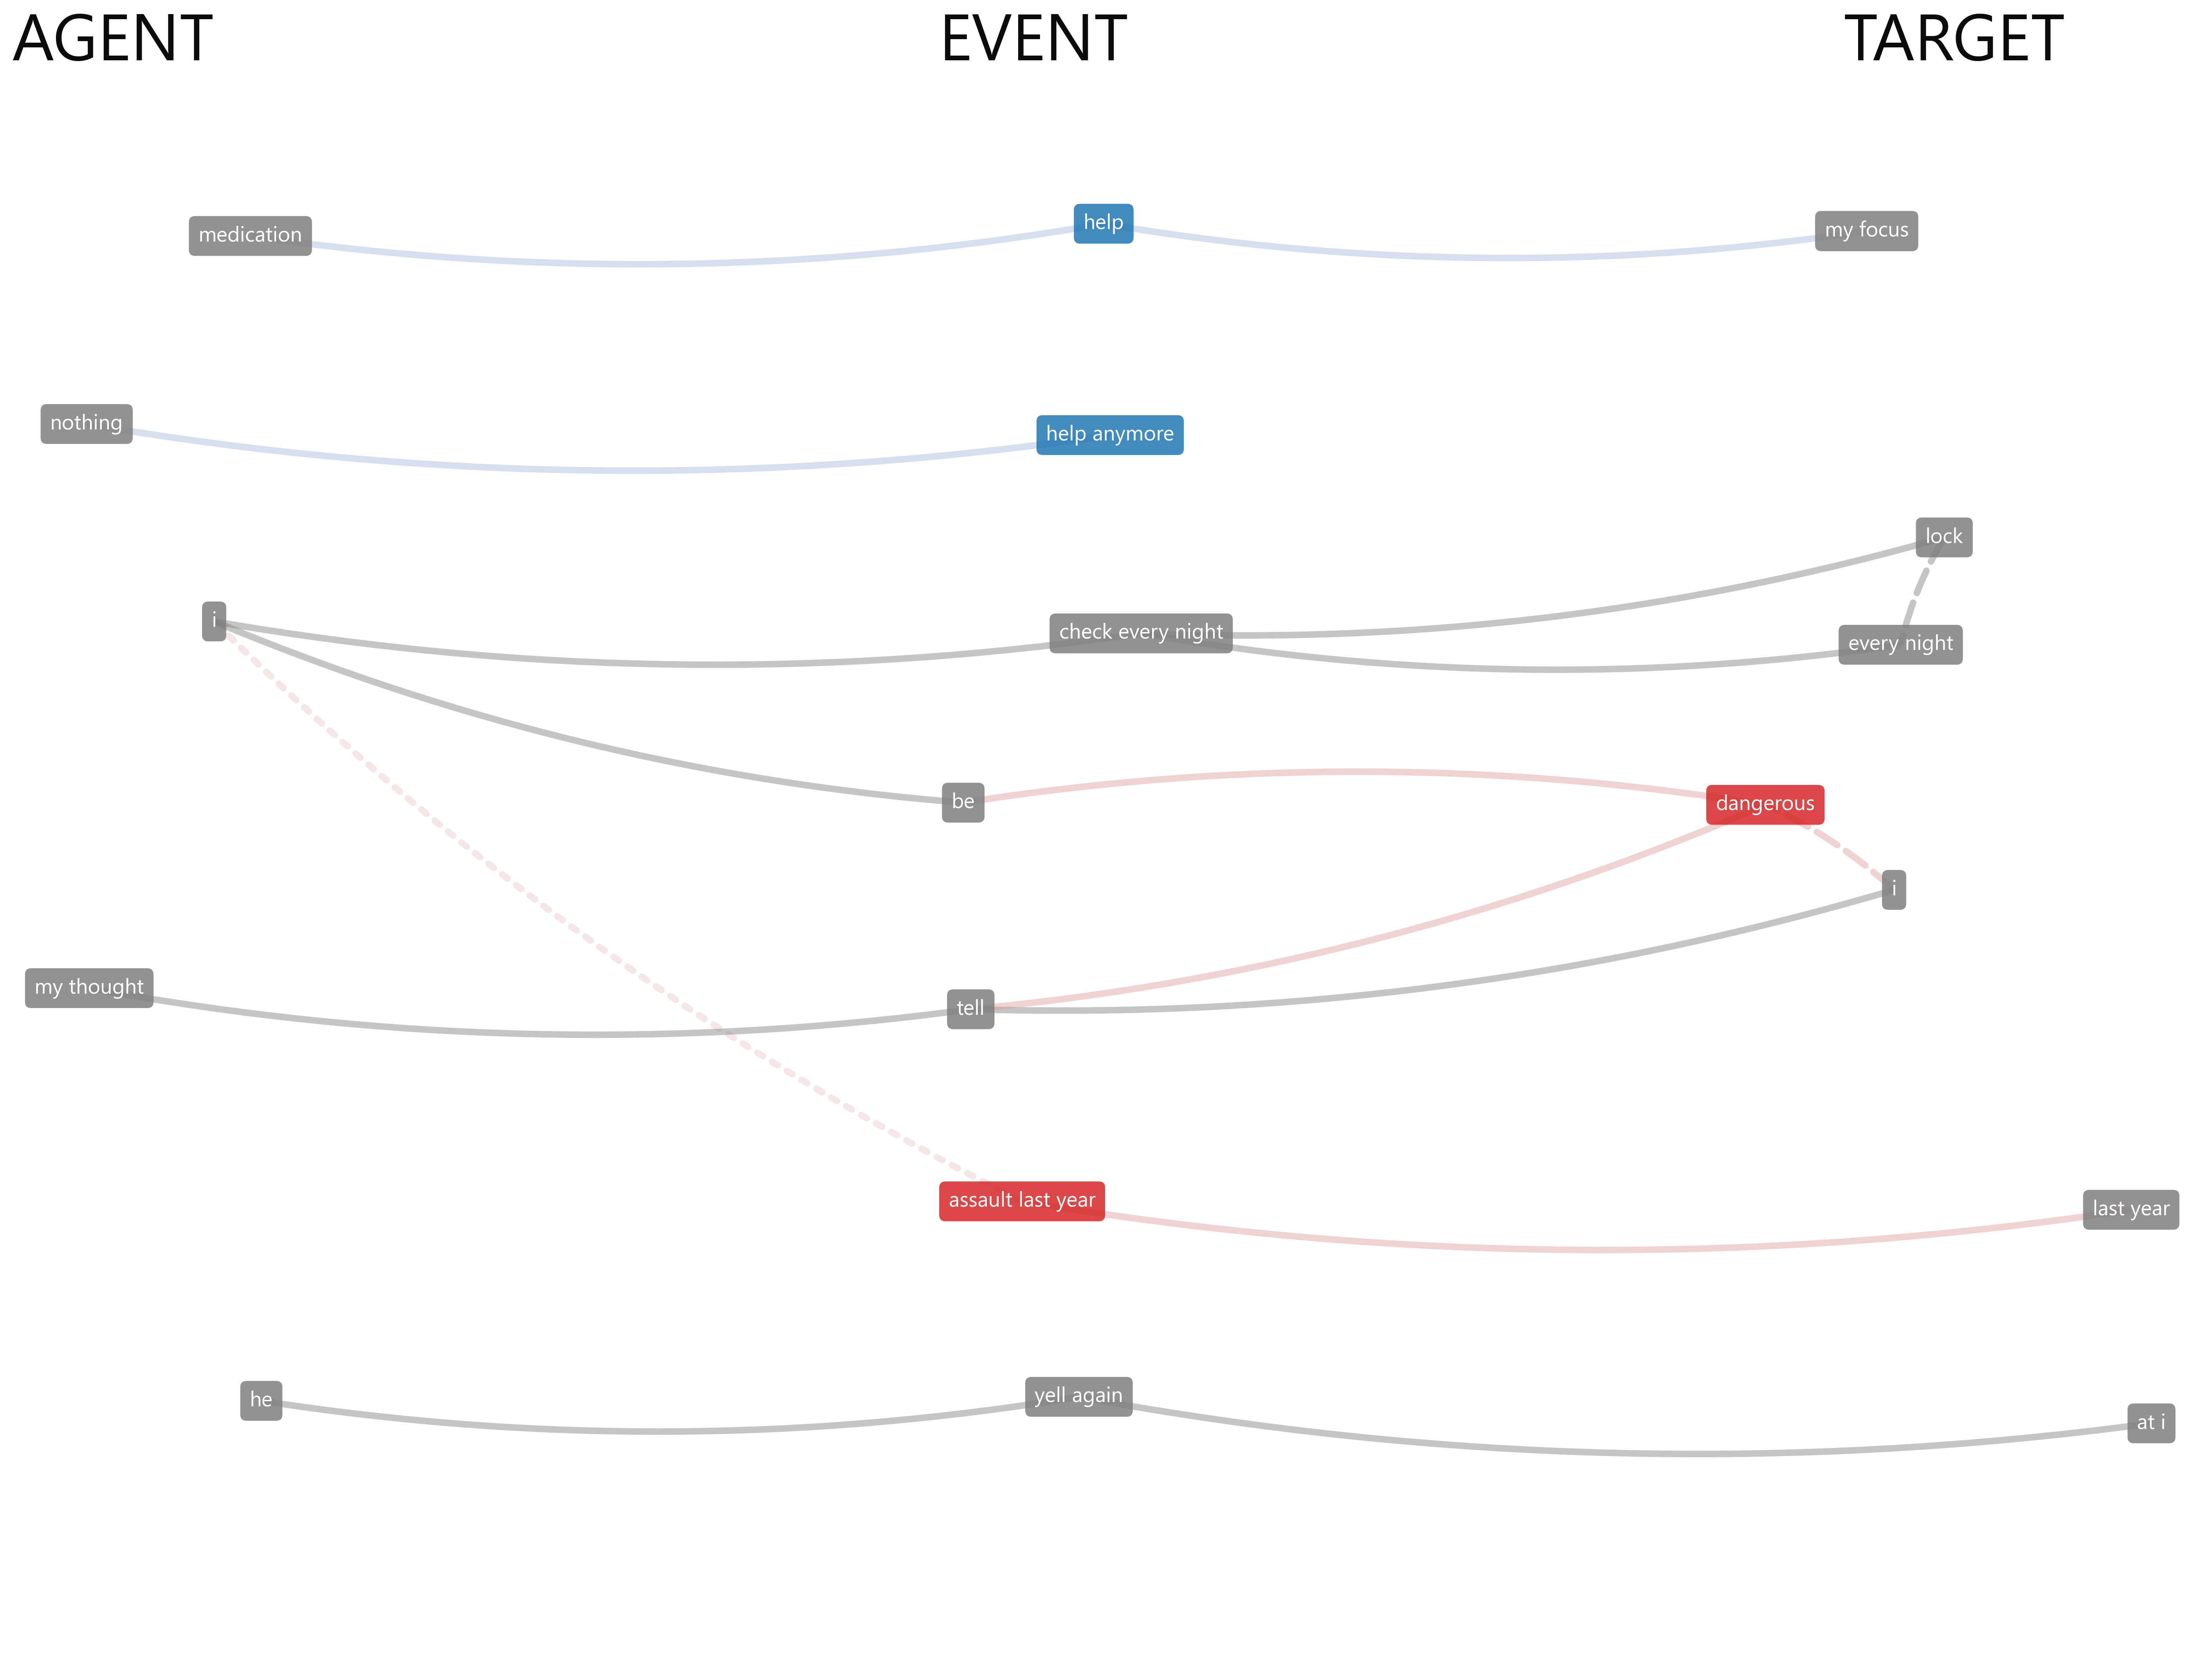
\includegraphics[width=0.92\textwidth]{figures/fig1_tea_example.png}
\caption{TEA network for six constructed sentences, drawn with the library's \texttt{plot\_svo\_graph} function: \textit{He yelled at me again. I was assaulted last year. My thoughts tell me that I am dangerous. I check the lock every night. Nothing helps anymore. The medication helps my focus.} Agents are on the left, events in the centre, targets on the right. The dashed link marks an agentless passive (``I'' $\to$ ``assault''), where the grammatical subject is the semantic patient. The library lemmatises pronouns, so ``me'' appears as ``i''. Node colour shows sentiment valence (red negative, blue positive, grey neutral).}
\label{fig:example}
\end{figure}

\subsection{Network structure}\label{sec:structure}

Structural metrics describe the shape of a post's network without looking at which words it contains. Some have a direct psychological reading. The first-person agent ratio is the share of actions whose doer is ``I'' or ``we''. The node type-token ratio and the number of unique nodes per word say how varied the entities in a story are, so low values mean that the writer keeps returning to the same few people or things. The largest strongly connected component and the clustering coefficient say how far the entities are woven into a single web of mutual relations rather than appearing in separate episodes.

To answer the first question we computed nine structural metrics on each TEA network: first-person agent ratio, size of the largest strongly connected component, triplets per word, density, average clustering, node type-token ratio, share of repeated edges, mean edge weight and unique nodes per word. Because these metrics depend on text length, each was regressed on log word count across the full sample and the residuals were analysed. We compared the four communities with Kruskal-Wallis tests, reported $\varepsilon^2$ as the effect size, and contrasted each community with the other three using Hedges' $g$ \citep{hedges1981}.

\subsection{Thematic concentration}\label{sec:rqa}

Some writers keep coming back to the same content. To measure this, each sentence was converted by a language model into a list of numbers (an embedding) such that sentences with similar meaning receive similar lists, whatever words they use: ``I can't stop checking the stove'' and ``I keep going back to make sure the gas is off'' have a similarity of 0.57 on a scale up to 1, while the first of them and ``My sister came to visit last weekend'' have 0.14. We then drew, for every post, a grid with the sentences along both sides and marked each pair of sentences whose meanings are close. The recurrence rate is the share of marked pairs, that is, how much of the post repeats content found elsewhere in it. Determinism is the share of marked pairs that fall in diagonal runs, which happens when a stretch of several consecutive sentences echoes an earlier stretch. Laminarity is the share that falls in vertical runs, which happens when several consecutive sentences all stay close to the same single sentence, that is, when the writer dwells on one point.

To measure how far a post keeps returning to the same content, we applied recurrence quantification analysis to the sequence of its sentences \citep{marwan2007}. Sentences were segmented with spaCy's statistical sentence segmenter, and sentences shorter than three words were dropped; 10,340 posts kept at least ten sentences (median 22). Each sentence was embedded with the sentence-transformer all-MiniLM-L6-v2 \citep{reimers2019}, and the whole analysis was repeated with all-mpnet-base-v2 as a check. We chose models trained for semantic similarity over averaged word vectors, whose similarities are driven largely by function words and pronouns and therefore track style as much as content.

Two sentences counted as recurrent when the cosine similarity of their embeddings exceeded a threshold. In the main analysis the threshold was global, set so that the recurrence rate pooled over 500 random posts was 10\% (0.384 for MiniLM, 0.400 for mpnet), and we repeated it with thresholds giving 5\% and 15\%. From each recurrence matrix we derived the recurrence rate, determinism, laminarity, trapping time, mean and maximum diagonal line length, and the entropy of diagonal line lengths. With a global threshold the recurrence rate varies between posts, and the other measures partly follow it. We therefore also used a per-post threshold that fixed each post's recurrence rate at 10\%. This separates the sequential structure of recurrence, whether similar sentences come in runs, from how similar a post's sentences are overall. Metrics were regressed on the log number of sentences and analysed with the same tests as the network metrics, with the false discovery rate controlled across all recurrence tests.

\subsection{Content signatures and classification}\label{sec:content}

We wanted to know which words are typical of each community and whether a computer can tell which community a post comes from. The second question is a way of measuring information. If a statistical model can guess the community from some description of the posts, that description captures something that differs between communities; if it guesses no better than chance, it does not. Accuracy is the share of posts assigned to the right community, which would be 25\% by chance with four communities. The AUC is the probability that the model rates a post from a given community as more likely to belong there than a post from elsewhere, from .50 (chance) to 1 (perfect). Each model was tested on posts it had not seen during training (cross-validation), so that it could not succeed by memorising the data.

To describe what distinguishes the communities, we counted for each community the number of posts in which a head word appeared in a given role and compared these counts with the other three communities using weighted log-odds ratios with an informative Dirichlet prior \citep{monroe2008}. Counting posts rather than tokens prevents a single long post from dominating a term. Only words occurring in at least 30 posts were considered.

To test whether roles add information, we trained multinomial logistic regression classifiers on TF-IDF features under five-fold stratified cross-validation, using a balanced subsample of 1,865 posts per community (the size of the smallest community) and the same folds for every feature set. The feature sets were: the raw words of the post; TEA head words without role labels; the same head words labelled by role (e.g. \texttt{A\_thought} versus \texttt{T\_thought}); each role on its own; and raw words plus role-labelled heads. Paired predictions were compared with exact McNemar tests. Two further classifiers used the nine residualised network metrics and the seven recurrence metrics of Section~\ref{sec:rqa} with the log number of sentences.

\subsection{Coding agency}\label{sec:coding}

To compare agency between communities we first had to know what kind of entity occupies each position: the narrator, another person, a thought, a medication, a span of time. Every word in an Agent or Target position was therefore sorted into a category using two fixed lists that were chosen before looking at the results. Pronouns were sorted by grammar (\textit{I}, \textit{he/she}, \textit{they}, and so on). All other words were sorted with WordNet, a large reference dictionary that files English nouns under 26 broad headings such as persons, feelings, cognition (thoughts, memories, ideas), artifacts (objects made by people, including medication), the body and time.

For the agency analysis we kept only the slots attached directly to an event: the head of each Agent in an Agent$\to$Event link and the head of each Target in an Event$\to$Target link. Links between two agents or two targets (coordination and modifier chains) were excluded. This gave 2,021,601 slots, 959,884 agents and 1,061,717 targets, with a median of 152 slots per post.

Each head word was assigned to one category by a fixed procedure. Pronouns were first sorted into closed grammatical classes: the self (\textit{I, me, myself, we, us}), \textit{you}, \textit{he/she} (with \textit{him, her}), \textit{they} (with \textit{them}), demonstratives and \textit{it}, absolutist pronouns (\textit{everyone, everybody, everything, nobody, nothing, none, all}) and other indefinites (\textit{someone, anything}, etc.). Every other word was assigned the lexicographer file, or supersense, of its most frequent noun sense in WordNet \citep{miller1995,ciaramita2003}, for example \texttt{noun.person}, \texttt{noun.cognition} or \texttt{noun.artifact}. The categories were therefore defined by an external taxonomy and not by inspecting the data. First-sense assignment is noisy for individual words (``med'' is filed under communication), but the noise is the same across communities.

Agentless passives were then handled explicitly. In the main analysis the subject of every link flagged \texttt{passive\_approx} was moved from the Agent to the Target role, so that ``I was assaulted'' counts the narrator as the one affected. Results without this correction are reported for comparison.

\subsection{Agentivity given mention}\label{sec:agentivity}

For each kind of entity we asked: when it appears in a sentence, how often is it the one acting rather than the one acted upon? We call this its agentivity. A community could mention the narrator very often and still rarely make the narrator act, so how often something is mentioned and how often it acts are kept separate. The comparison is expressed as an odds ratio. An odds ratio of 1 means that, in a given community, an entity acts as often as one would expect from how agentive that entity is elsewhere and how agentive that community's writing is overall. Values above 1 mean it acts more often than expected, values below 1 less often. An odds ratio of 0.62, for example, means that the odds of the entity being the actor are 38\% lower than expected.

For a category $c$ in a post, agentivity is the share of its slots that are Agent slots. The question of interest is whether agentivity for a category is higher or lower in one community than in the others after accounting for how agentive each community is overall. For every pair of category $c$ and community $k$ we fitted a binomial generalised linear model on slot counts aggregated by post:
\begin{equation}
\operatorname{logit} P(\text{Agent}) = \beta_0 + \beta_1\,\mathrm{cat}_c + \beta_2\,\mathrm{com}_k + \beta_3\,\mathrm{cat}_c \times \mathrm{com}_k ,
\end{equation}
where $\mathrm{cat}_c$ marks the slots of category $c$ and $\mathrm{com}_k$ marks posts from community $k$. The odds ratio $e^{\beta_3}$ is the extra agentivity of category $c$ in community $k$ beyond what the category and the community imply on their own. Because the model conditions on mention, it is not affected by how often a community talks about a given entity. Standard errors were clustered by author, with each post by a deleted account treated as its own cluster. We tested nine categories chosen for their theoretical relevance and frequency (self, \textit{he/she}, \textit{they}, persons, absolutist pronouns, and the cognition, time, body and artifact supersenses) in each of the four communities, and controlled the false discovery rate across the 36 tests with the Benjamini-Hochberg procedure \citep{benjamini1995}.

\subsection{Robustness checks}\label{sec:robust}

Some of the agency results could in principle come from choices made in the analysis: how passive sentences are treated, the fact that some people wrote several posts, or chance variation within the sample. The checks below test each of these.

We repeated the agentivity models (a) without the passive correction, (b) with standard errors clustered by post, (c) on a sample with one randomly chosen post per author (9,353 posts), and (d) separately in two random halves of the posts, reporting the correlation of the log odds ratios across halves.

\subsection{Reading the statistics}

With more than ten thousand posts almost every difference is statistically significant, so the size of an effect matters more than its $p$-value. Differences between groups are reported as Hedges' $g$, the difference in means expressed in standard deviations; by common convention 0.2 is a small effect, 0.5 a medium one and 0.8 a large one \citep{cohen1988}. In this paper $g$ always compares one community with the other three together. $\varepsilon^2$ is the share of the variation between posts that is explained by which community they come from; .04 means 4\%. Odds ratios are explained in Section~\ref{sec:agentivity}, and their 95\% confidence intervals give the range of values compatible with the data. Because many tests were run, $p$-values were adjusted with the Benjamini-Hochberg procedure, which limits the expected share of false positives among the results called significant.

\subsection{Ethics}

All posts were publicly available at the time of collection and were analysed in aggregate. We do not quote posts or report usernames. Example sentences in the figures are constructed, and the data-driven network figures show only triplets that occur in at least three different posts.

% =====================================================================
\section{Results}

\subsection{Network structure separates the communities poorly}

The first question was whether the overall shape of the who-does-what-to-whom maps differs between communities, regardless of which words fill them. It does, but only slightly: knowing the shape of a post's network helps little in guessing where it was written.

All nine network metrics differed across communities after correction, which is unsurprising with ten thousand posts, but the differences were small. The largest effect sizes were $\varepsilon^2 = .016$ for the first-person agent ratio and $.013$ for both the node type-token ratio and the largest strongly connected component; the others ranged from $.004$ to $.012$. In one-versus-rest contrasts, the largest effects were a higher first-person agent ratio in r/depression ($g = 0.31$), a lower node type-token ratio in r/OCD ($g = -0.24$) and a smaller strongly connected component in r/ADHD ($g = -0.24$). A classifier using the nine metrics identified the community of a post 33.6\% of the time, against a chance level of 25\% (macro-averaged AUC $= .60$). The way a post's network is shaped says something about where it was written, but not much.

\subsection{Posts in r/OCD are the most thematically concentrated, posts in r/depression the least}

Posts in r/OCD returned to the same content most often: their sentences were more often close in meaning to other sentences in the same post. Posts in r/depression did so the least and ranged over more subjects. Posts in r/ptsd and r/ADHD were in between.

With MiniLM and the 10\% threshold, recurrence rate was highest in r/OCD (mean .18; $g = 0.36$ against the other three communities) and lowest in r/depression (.12; $g = -0.39$), with r/ptsd (.14; $g = -0.08$) and r/ADHD (.16; $g = -0.01$) in between (Figure~\ref{fig:concentration}A). Laminarity (r/OCD $g = 0.31$, r/depression $g = -0.38$), determinism ($0.26$ and $-0.28$) and entropy ($0.22$ and $-0.27$) followed the same pattern. Recurrence rate explained 4.0\% of the variance between communities ($\varepsilon^2 = .040$), more than any network metric. The pattern held with thresholds giving 5\% and 15\% recurrence (r/OCD $g$ from 0.32 to 0.41, r/depression from $-0.43$ to $-0.35$) and with mpnet ($0.33$ and $-0.37$ at 10\%). Across all metrics, thresholds and communities, the effect sizes from the two models correlated at $r = .99$.

With the per-post threshold the differences disappeared (all $|g| \leq 0.10$, $\varepsilon^2 \leq .002$; Figure~\ref{fig:concentration}B). Posts in r/OCD do not return to a theme in longer or more regular runs than other posts; their sentences are closer to one another in meaning overall. We therefore describe the result as thematic concentration rather than recurrence in a dynamical sense. A classifier using the seven recurrence metrics reached 32.6\% accuracy (macro AUC $= .60$), so concentration, like network structure, separates the communities on average but not post by post.

\begin{figure}[t]
\centering
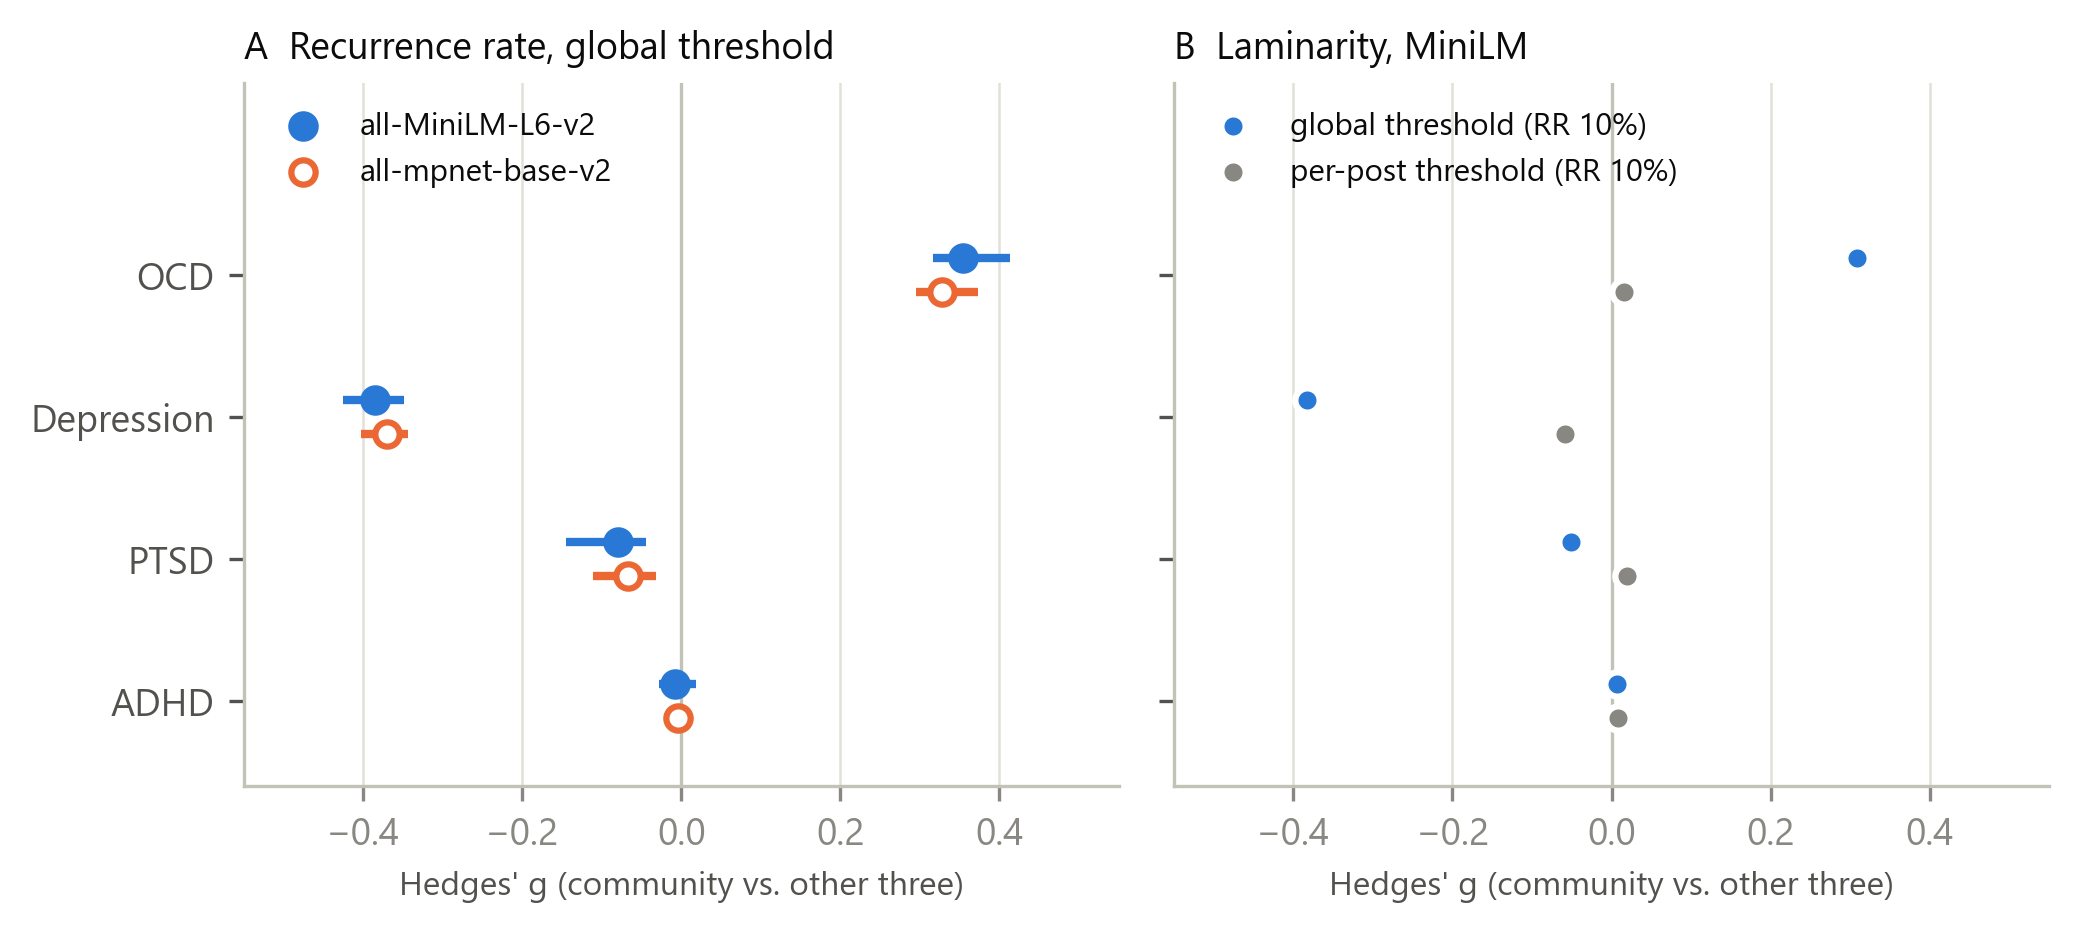
\includegraphics[width=\textwidth]{figures/fig7_thematic_concentration.png}
\caption{Thematic concentration. Effect sizes (Hedges' $g$) for each community against the other three, after adjusting for the number of sentences. (A) Recurrence rate with a global threshold set to a pooled recurrence rate of 10\%, for two sentence-transformer models; bars span the results for thresholds giving 5\% and 15\%. (B) Laminarity with the global threshold and with a per-post threshold that fixes each post's recurrence rate at 10\%; once overall similarity is held constant, the communities no longer differ.}
\label{fig:concentration}
\end{figure}

\subsection{Network content separates them well, but roles add nothing to classification}

The words that fill the networks differ between communities far more than their shape does, mostly because each community talks about different things: medication in r/ADHD, abuse in r/ptsd, intrusive thoughts and checking in r/OCD. Knowing whether a word appears as the doer or as the one done to, however, did not help a computer recognise the community any better than knowing that the word appears at all.

The content of the networks was far more informative. Figure~\ref{fig:content} shows the head words most specific to each community in the Agent and Event roles. In r/OCD the most distinctive agents were \textit{thought}, \textit{fear}, \textit{obsession}, \textit{brain} and \textit{mind}, and the most distinctive events were \textit{obsess}, \textit{touch}, \textit{worry}, \textit{wash}, \textit{ruminate} and \textit{check}. In r/depression they were \textit{life}, \textit{family}, \textit{world}, \textit{nobody}, \textit{everyone}, \textit{nothing} and \textit{future} as agents, and \textit{care (anymore)}, \textit{die}, \textit{live}, \textit{wish} and \textit{hate} as events. In r/ptsd they were \textit{trauma}, \textit{he}, \textit{abuse}, \textit{man}, \textit{boyfriend}, \textit{father} and \textit{police}, and \textit{abuse}, \textit{trigger}, \textit{scream}, \textit{assault} and \textit{dissociate}. In r/ADHD they were \textit{medication}, \textit{doctor}, \textit{task}, \textit{work} and \textit{psychiatrist}, and \textit{focus}, \textit{diagnose}, \textit{prescribe}, \textit{study} and \textit{procrastinate}.

\begin{figure}[t]
\centering
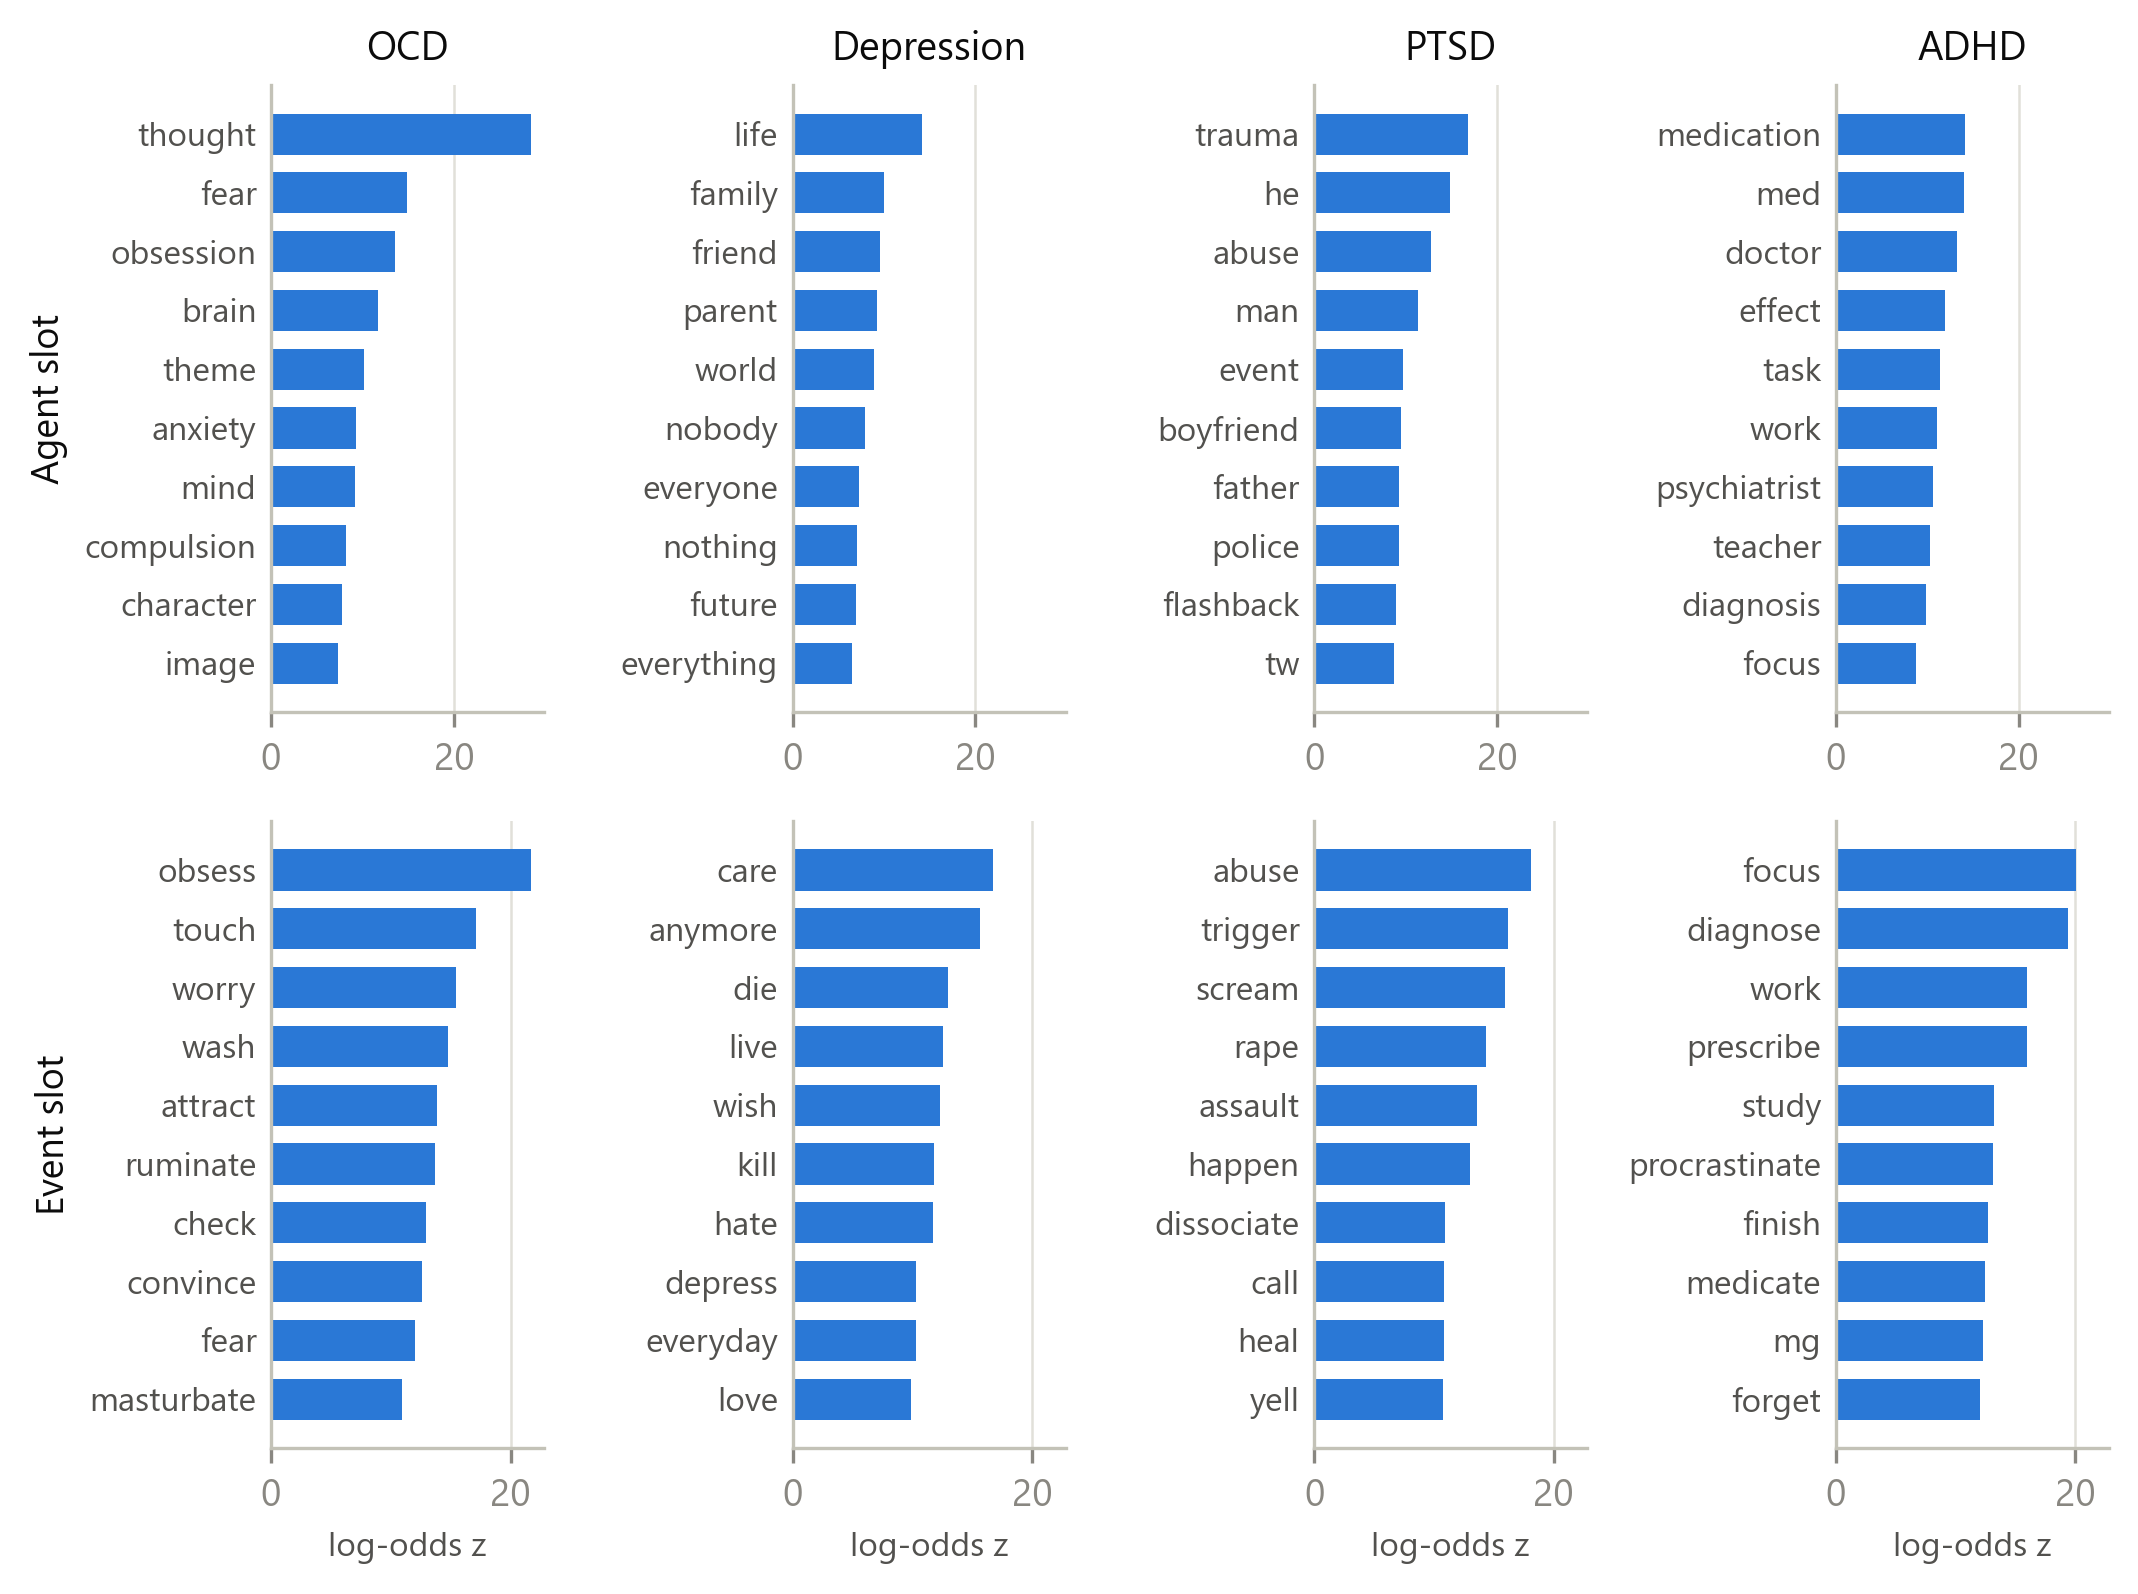
\includegraphics[width=\textwidth]{figures/fig6_content_signatures.png}
\caption{Head words most specific to each community in the Agent (top) and Event (bottom) roles, ranked by the $z$-score of the weighted log-odds ratio against the other three communities \citep{monroe2008}. Counts are numbers of posts. Condition names were removed before the analysis. spaCy lemmatises \textit{raped} as \textit{rap}; the label is shown as \textit{rape}.}
\label{fig:content}
\end{figure}

A classifier using role-labelled head words reached 81.7\% accuracy (macro AUC $= .954$; Table~\ref{tab:ablation}). The role labels, however, did not help. The same head words without labels did as well (82.1\%; McNemar $p = .17$), and the raw words of the post did better (84.8\%; $p < .001$). Adding role-labelled heads to the raw words left accuracy unchanged (85.0\% versus 84.8\%; $p = .39$). Taken one at a time, targets carried the most information (78.2\%), then events (69.3\%), then agents (61.4\%). For telling the communities apart, then, TEA networks are a compressed and slightly lossy version of the text. Their content signal is a topical signal, which is what one would expect from communities that discuss medication, abuse or intrusive thoughts.

\begin{table}[t]
\centering
\caption{Classification of posts into the four communities. Balanced subsample of 1,865 posts per community, five-fold cross-validation with the same folds for every feature set. Chance accuracy is 25\%. $^a$Balanced subsample of the 10,340 posts with recurrence data.}
\label{tab:ablation}
\small
\begin{tabular}{@{}lcc@{}}
\toprule
Features & Accuracy & Macro AUC \\
\midrule
9 network-structure metrics & .336 & .604 \\
7 recurrence metrics (MiniLM)$^a$ & .326 & .603 \\
Raw words of the post & .848 & .968 \\
TEA head words, no roles & .821 & .957 \\
TEA head words with roles & .817 & .954 \\
\quad Agent slot only & .614 & .840 \\
\quad Event slot only & .693 & .892 \\
\quad Target slot only & .782 & .941 \\
Raw words + TEA heads with roles & .850 & .968 \\
\bottomrule
\end{tabular}
\end{table}

\subsection{The same mentions, different roles}

The central analysis concerns position. Once the narrator, other people or thoughts are mentioned, are they the ones acting or the ones acted upon? The four communities answered this in different ways.

Overall agentivity was almost identical in the four communities, between 45.4\% and 45.9\% of slots, so none of the differences below comes from one community simply using more agents.

The narrator is the clearest case (Figure~\ref{fig:mention}). The self accounted for 28.7\% of slots in r/OCD, 28.6\% in r/ptsd and 28.6\% in r/ADHD, and somewhat more (31.3\%) in r/depression. The role it took varied a good deal more than its frequency. When the self appeared, it was the agent in 85.5\% of cases in r/OCD and 85.4\% in r/ADHD, but in 82.0\% in r/depression and 79.2\% in r/ptsd. Other people showed the mirror image. Person nouns (\textit{mom}, \textit{friend}, \textit{therapist}, \textit{boyfriend}) were mentioned most in r/ptsd and least in r/ADHD and r/OCD, and when they were mentioned they were agents in 38.6\% of cases in r/ptsd against 26.9\% in r/OCD. The pronoun \textit{they} followed the same pattern (69.8\% versus 59.5\%).

\begin{figure}[t]
\centering
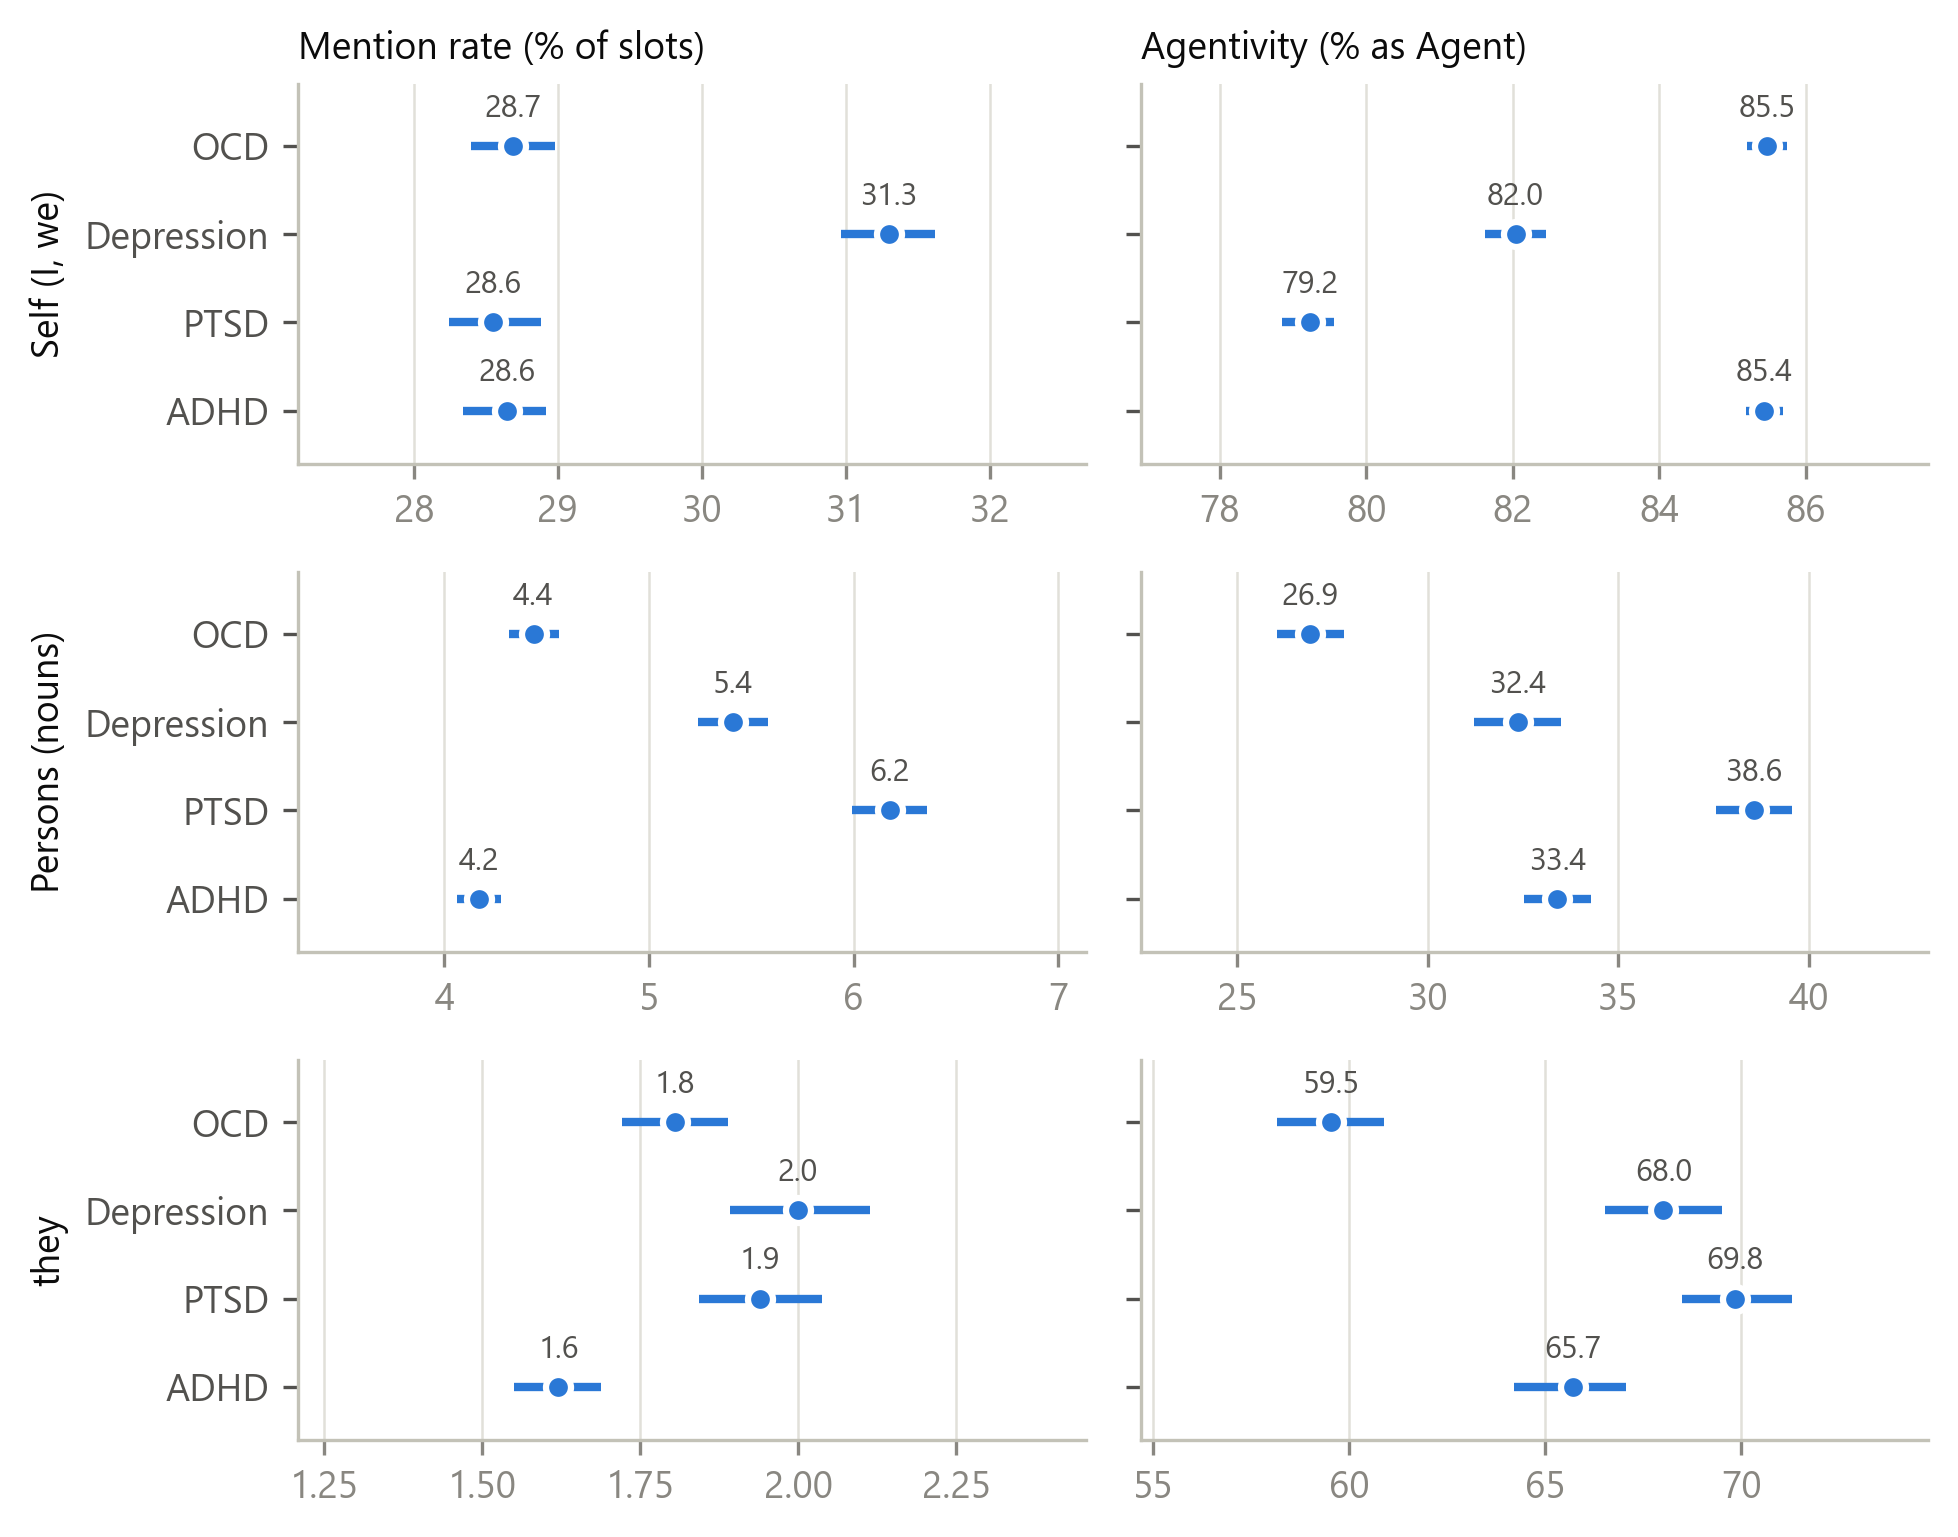
\includegraphics[width=0.92\textwidth]{figures/fig3_mention_vs_agentivity.png}
\caption{How often an entity is mentioned (left) and, when mentioned, how often it is the Agent rather than the Target (right), for the self, person nouns and \textit{they}. Passive-corrected slots. Points are pooled percentages, bars are 95\% bootstrap intervals over posts (1,000 resamples). In r/OCD, r/ptsd and r/ADHD the self is mentioned at the same rate but cast as agent at very different rates.}
\label{fig:mention}
\end{figure}

The interaction models put these differences on a common scale, where an odds ratio above 1 means that an entity is the one acting more often than expected and below 1 less often (Figure~\ref{fig:heatmap}; all odds ratios reported below are passive-corrected with errors clustered by author, and all are significant after Benjamini-Hochberg correction unless stated otherwise). They yield a profile for each community.

\paragraph{r/ptsd.} Writers in r/ptsd more often describe themselves on the receiving end of what happens, and other people as the ones doing it. The self was much less agentive than expected (OR = 0.62, 95\% CI 0.59--0.64), and other people were much more agentive: person nouns OR = 1.44 (1.36--1.52), \textit{they} OR = 1.32 (1.22--1.42). For \textit{he/she} the odds ratio was 1.05 (1.00--1.11, $p_\mathrm{BH} = .08$); these pronouns are agents most of the time in every community, but they were mentioned more than twice as often in r/ptsd (6.8\% of slots against 2.9--4.3\% elsewhere). Cognition nouns (OR = 0.93), time (0.87), the body (0.75) and artifacts (0.89) were less agentive than elsewhere.

\paragraph{r/OCD.} The profile was close to the reverse: the writer is the one acting even more often than elsewhere, other people act less often, and thoughts act more often than in the other communities. The self was more agentive (OR = 1.30, 1.25--1.35), while person nouns (OR = 0.66, 0.63--0.71), \textit{they} (0.69) and \textit{he/she} (0.80) were less so. Cognition nouns such as \textit{thought}, \textit{mind} and \textit{memory} were both mentioned more often (5.3\% of slots against 3.3--4.3\%) and, when mentioned, more often agents (OR = 1.13, 1.08--1.19). Absolutist pronouns (0.89) and time (0.80) were less agentive.

\paragraph{r/depression.} Here what stands out is that broad, impersonal things take the active role: time, and words such as ``nothing'' or ``nobody''. Time nouns (\textit{day}, \textit{year}, \textit{future}) were more agentive than in any other community (OR = 1.26, 1.16--1.38), as were absolutist pronouns (OR = 1.14, 1.05--1.23) and \textit{they} (1.14). The self was mentioned most often here but was slightly less agentive than average (OR = 0.94, 0.90--0.98). Artifacts (0.75) and the body (0.77) were rarely agents.

\paragraph{r/ADHD.} The writer acts often, and so do medication and the body. Artifacts, mostly medication, were more agentive than elsewhere (OR = 1.36, 1.27--1.46), and so was the body (OR = 1.48, 1.34--1.64). The self was as agentive as in r/OCD (OR = 1.32), and \textit{he/she} more agentive than expected (1.35). Person nouns and \textit{they} did not differ from the average.

\begin{figure}[t]
\centering
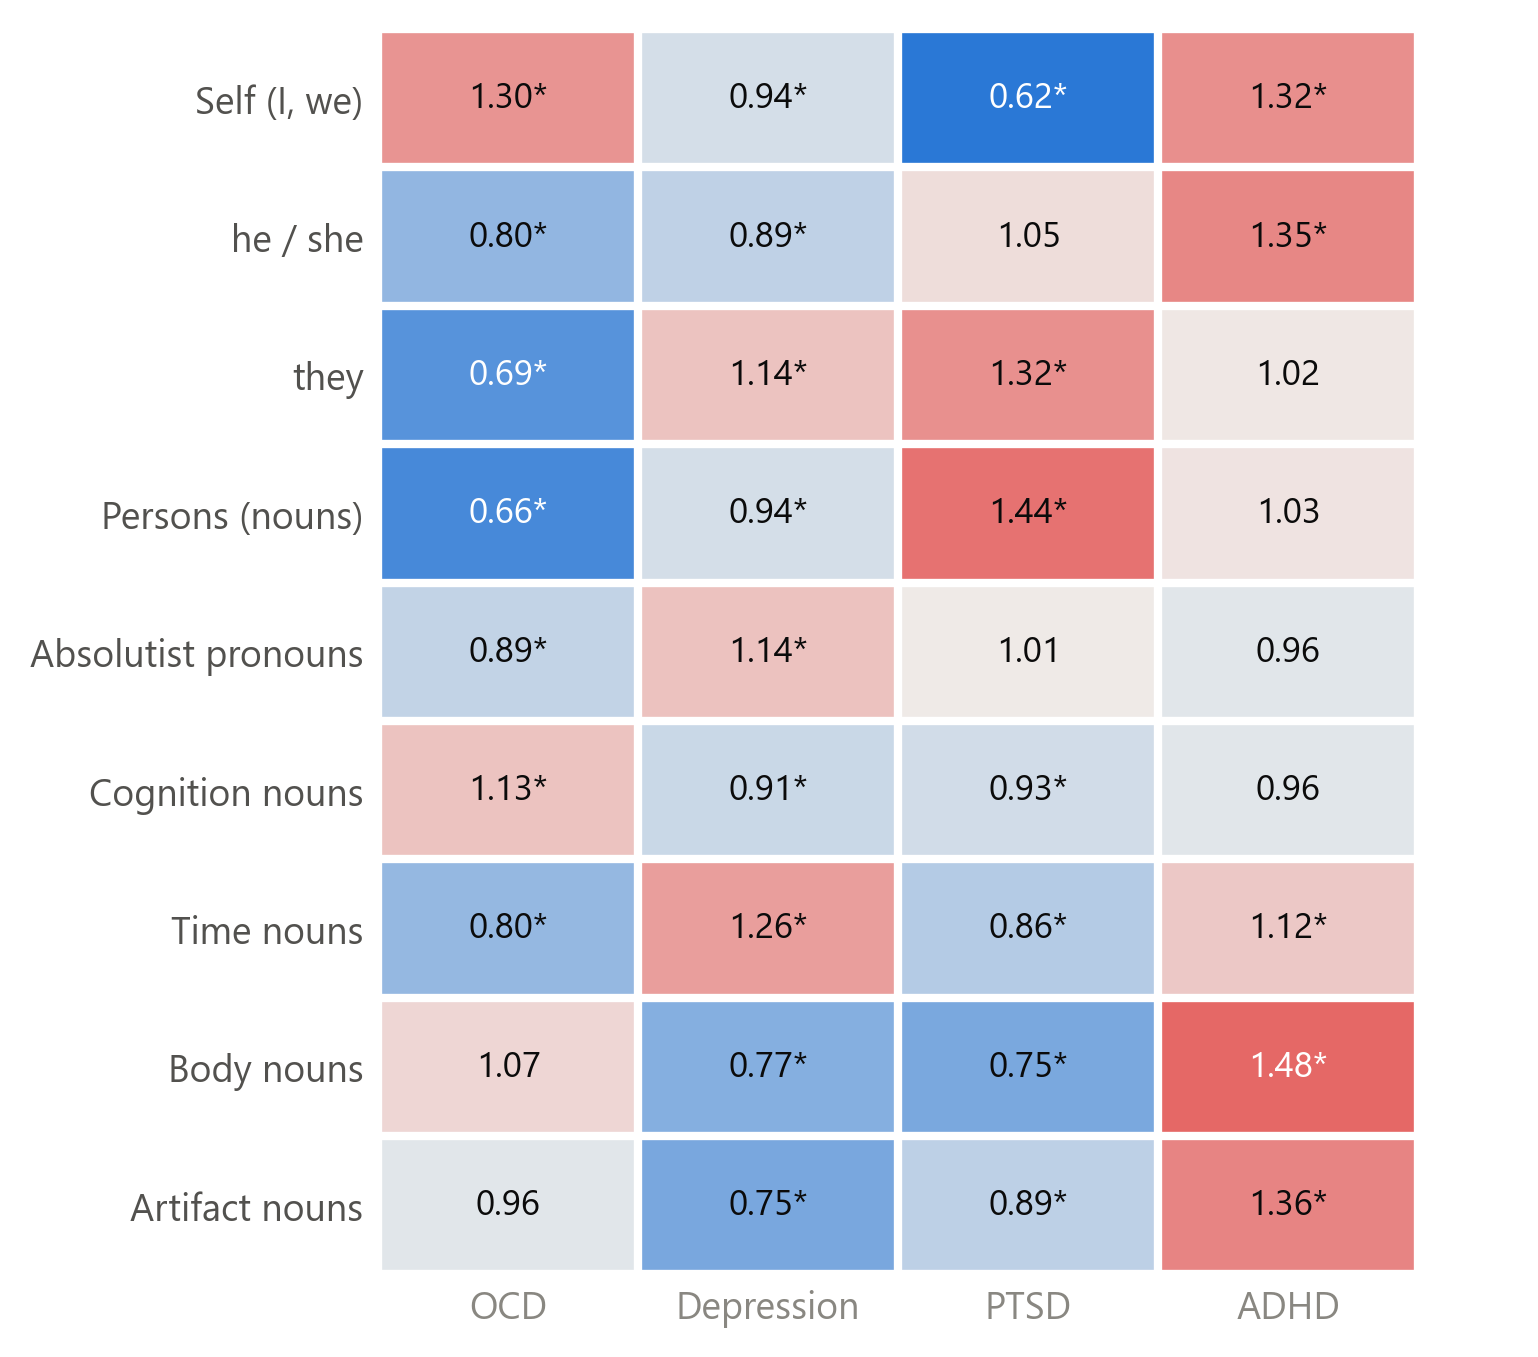
\includegraphics[width=0.62\textwidth]{figures/fig4_agentivity_heatmap.png}
\caption{Agentivity odds ratios for nine categories of entity in each community, from binomial models with a category $\times$ community interaction (passive-corrected slots, standard errors clustered by author). Values above 1 (red) mean the category is cast as Agent more often in that community than its overall frequency of agency and the community's overall agentivity would predict; values below 1 (blue) mean less often. Asterisks: $p_\mathrm{BH} < .05$ over 36 tests.}
\label{fig:heatmap}
\end{figure}

Plotting the agentivity of the self against that of other people places the four communities in different regions (Figure~\ref{fig:map}). r/ptsd sits alone in the quadrant where others act and the self is acted upon; r/OCD sits in the opposite corner; r/ADHD has an agentive self without suppressing others; r/depression lies near the centre on both axes, and its distinctive features lie elsewhere, in time and absolutist pronouns.

\begin{figure}[t]
\centering
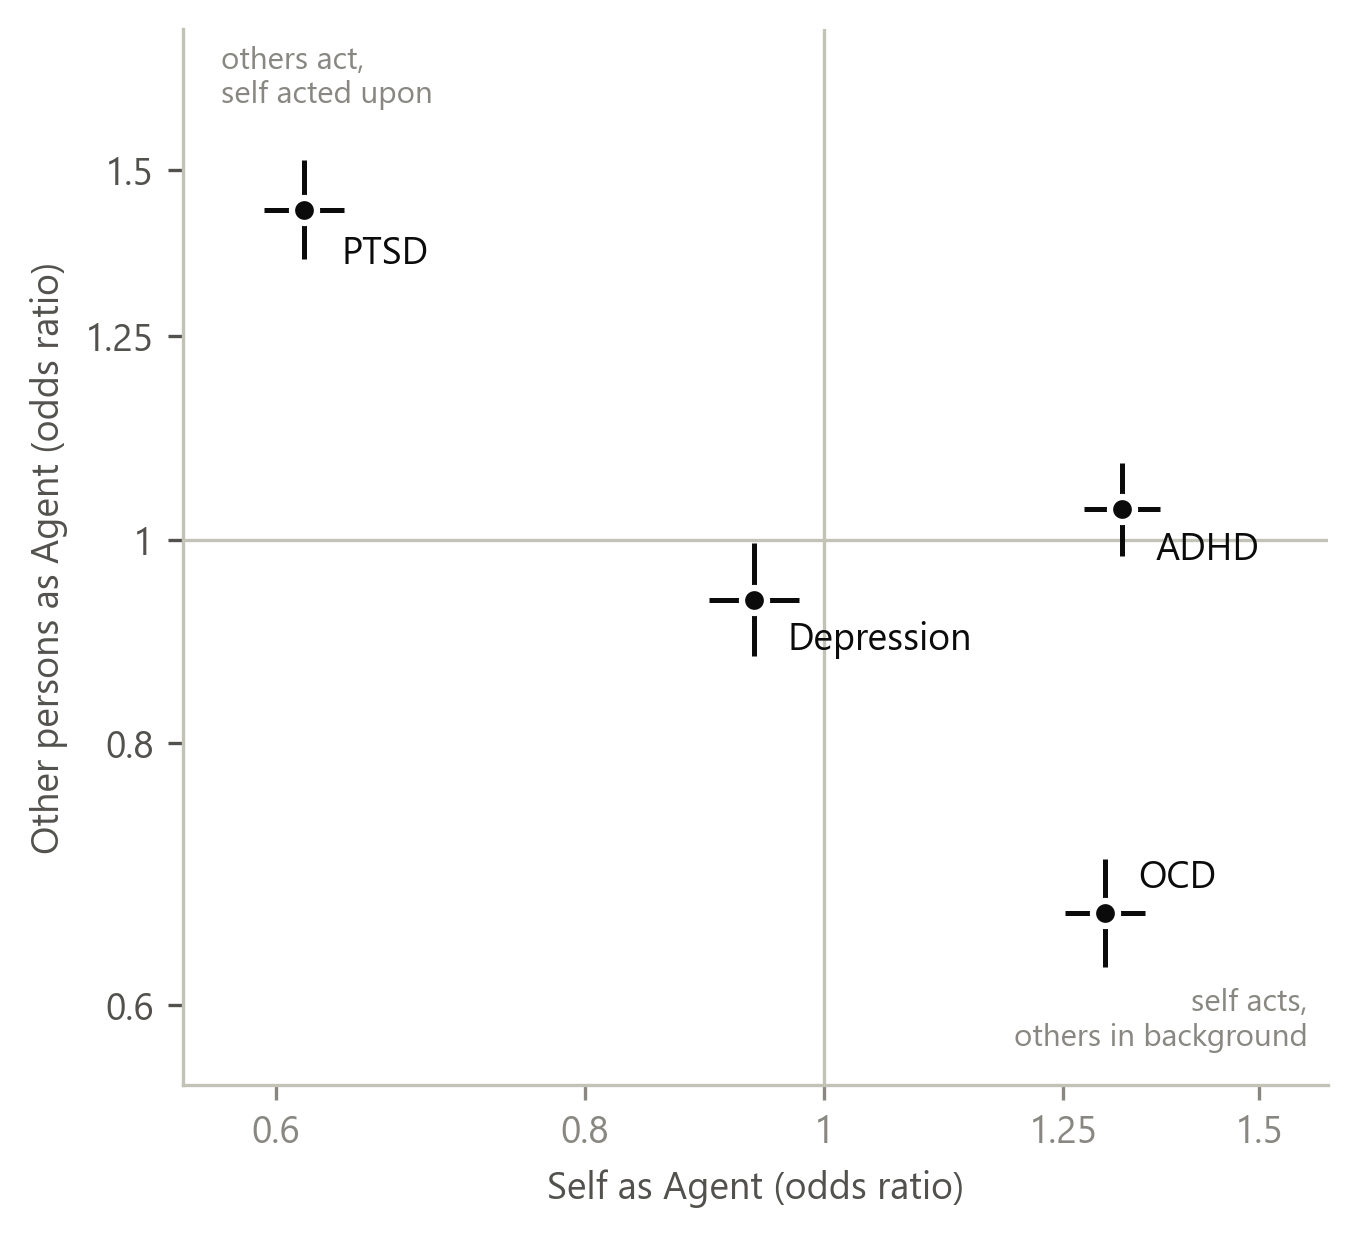
\includegraphics[width=0.55\textwidth]{figures/fig5_agency_map.png}
\caption{Agency map. Each community's odds ratio for the self as Agent (horizontal) against person nouns as Agent (vertical), with 95\% confidence intervals (author-clustered). Both axes are logarithmic; the grey lines mark an odds ratio of 1.}
\label{fig:map}
\end{figure}

Figure~\ref{fig:networks} shows what two of these profiles look like in the data. Across all 2,485 r/ptsd posts, the most frequent things \textit{he} did had the narrator as target: \textit{he} told the narrator something in 212 posts, and said, gave, asked, called, took, talked, loved, hit, left and hurt in 31 to 72 posts each. Across all 3,058 r/OCD posts, \textit{thought} as agent most often popped into the narrator's head (31 posts), told or bothered the narrator (15 each), felt real (13), came to mind (11), caused or gave anxiety, and ruined a life.

\begin{figure}[t]
\centering
\begin{subfigure}{0.49\textwidth}
\centering
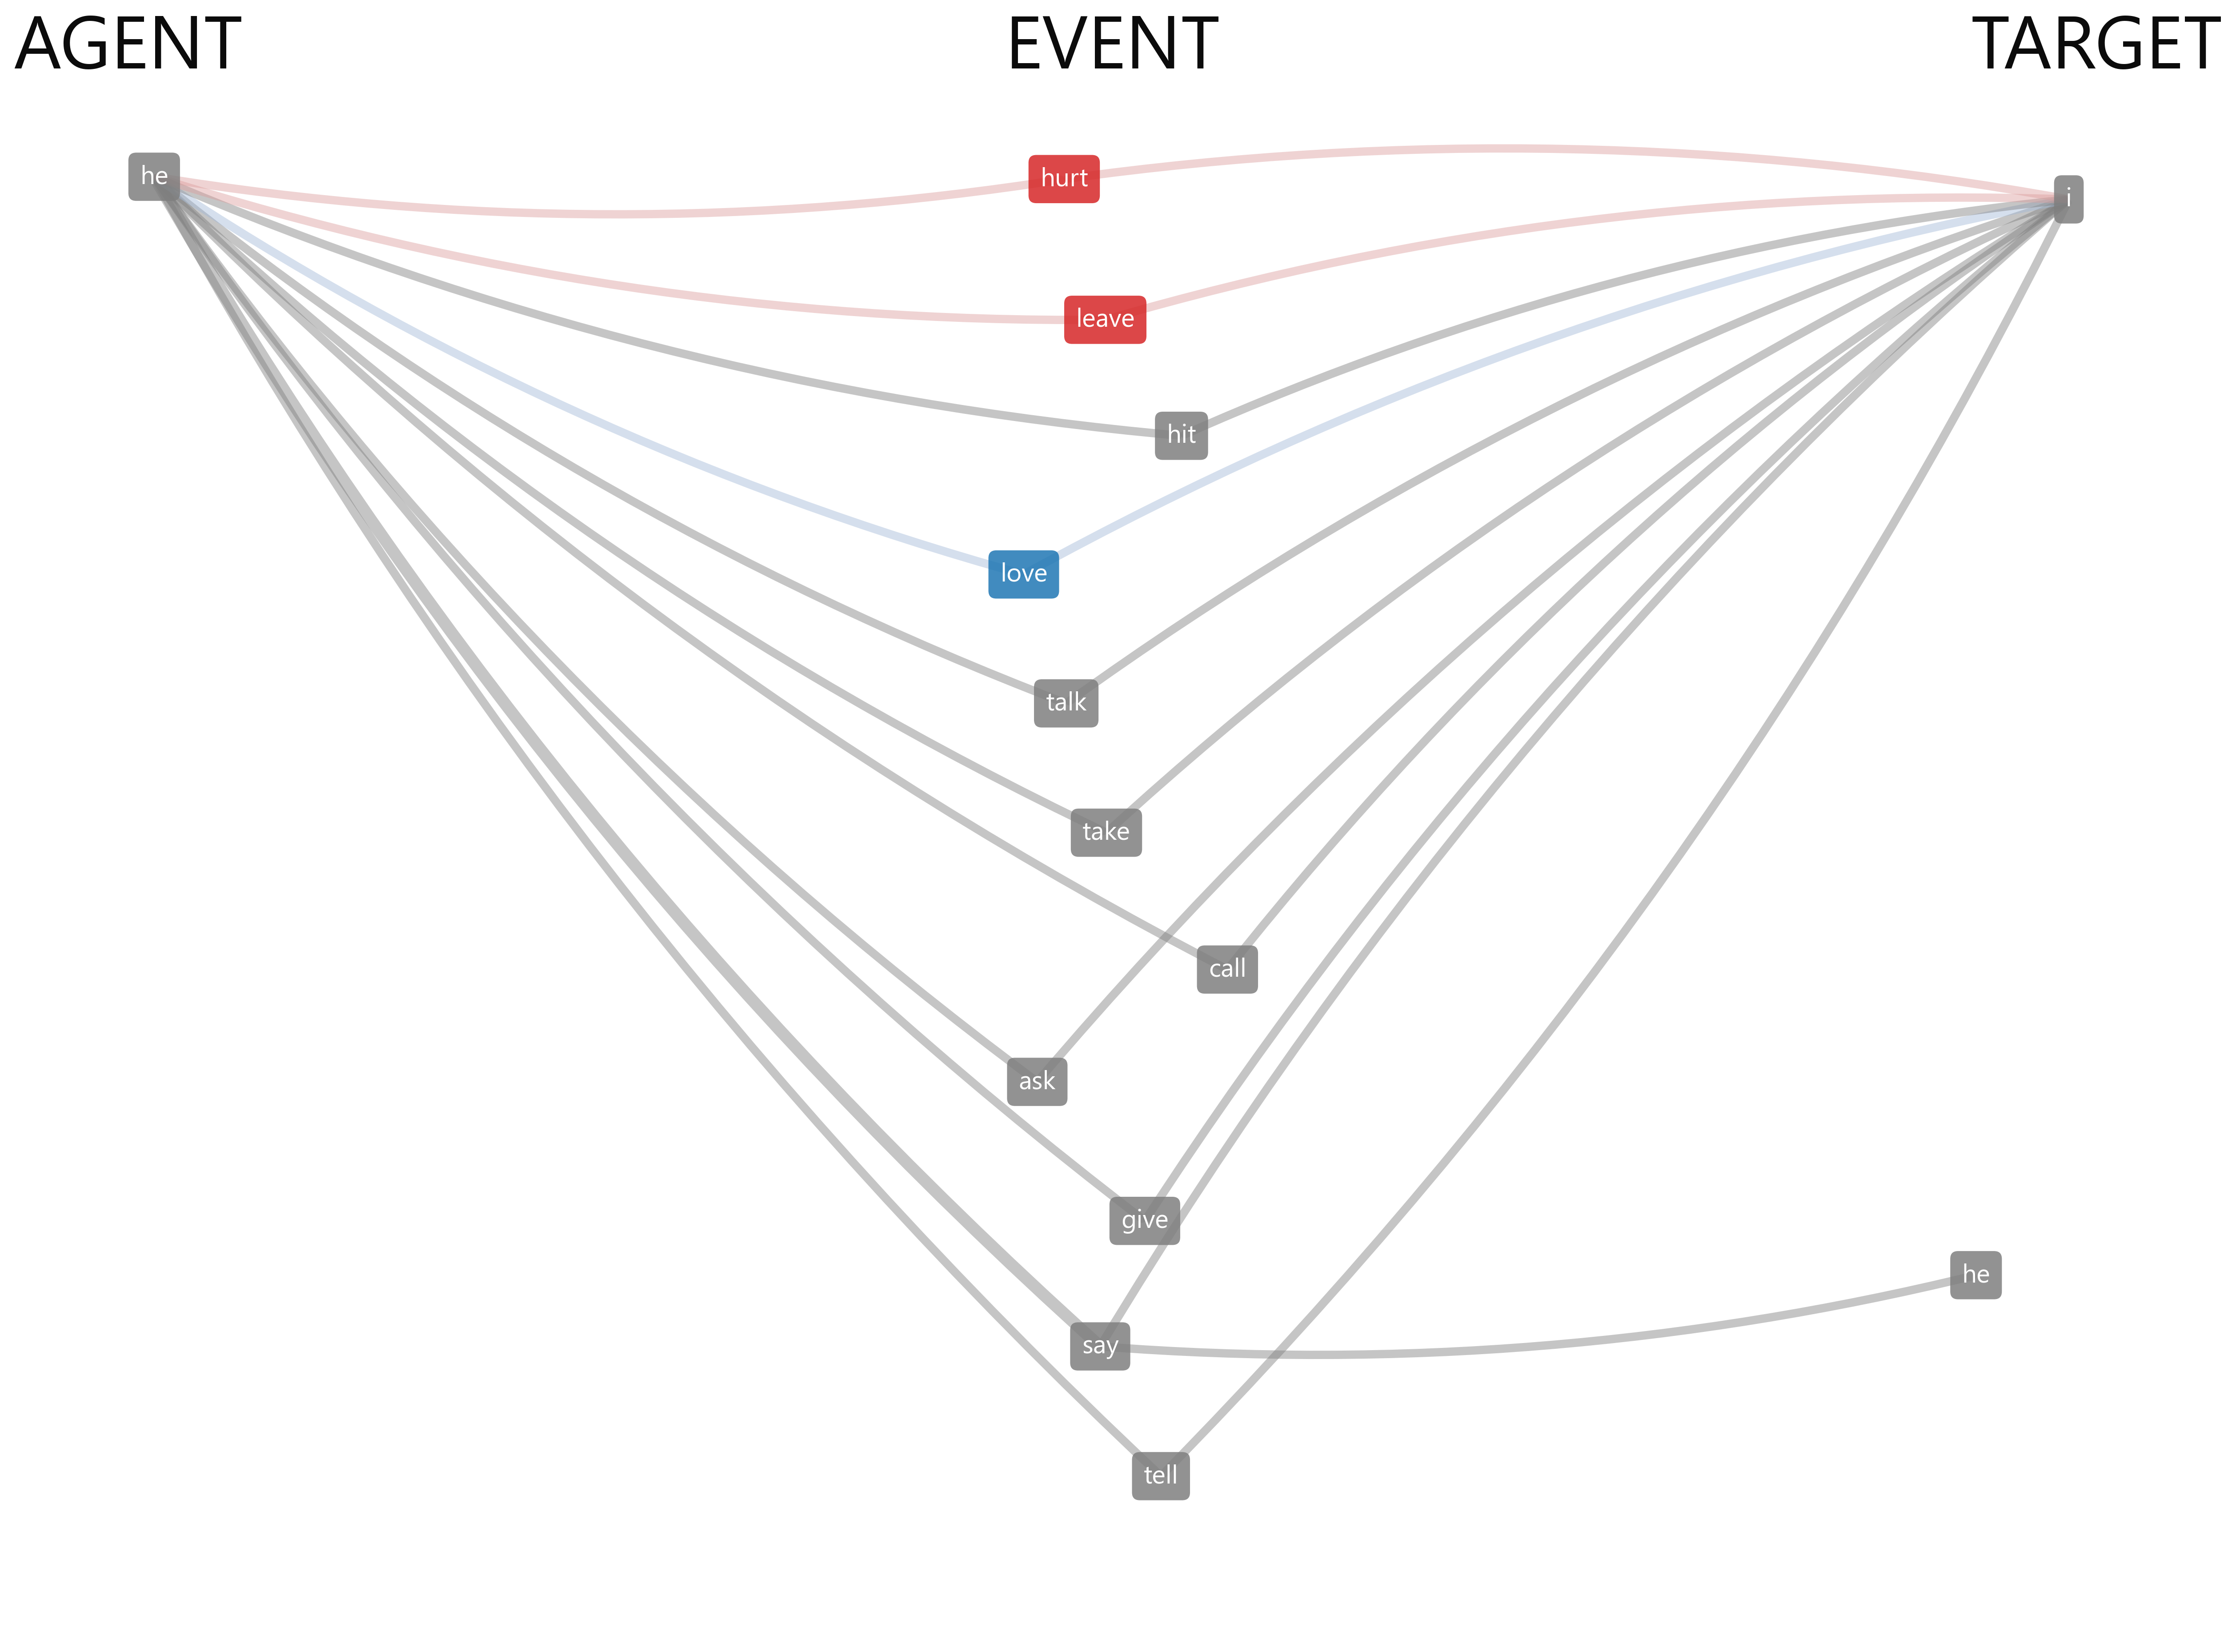
\includegraphics[width=\textwidth]{figures/fig2_tea_ptsd_he.png}
\caption{r/ptsd, agent \textit{he}}
\end{subfigure}
\hfill
\begin{subfigure}{0.49\textwidth}
\centering
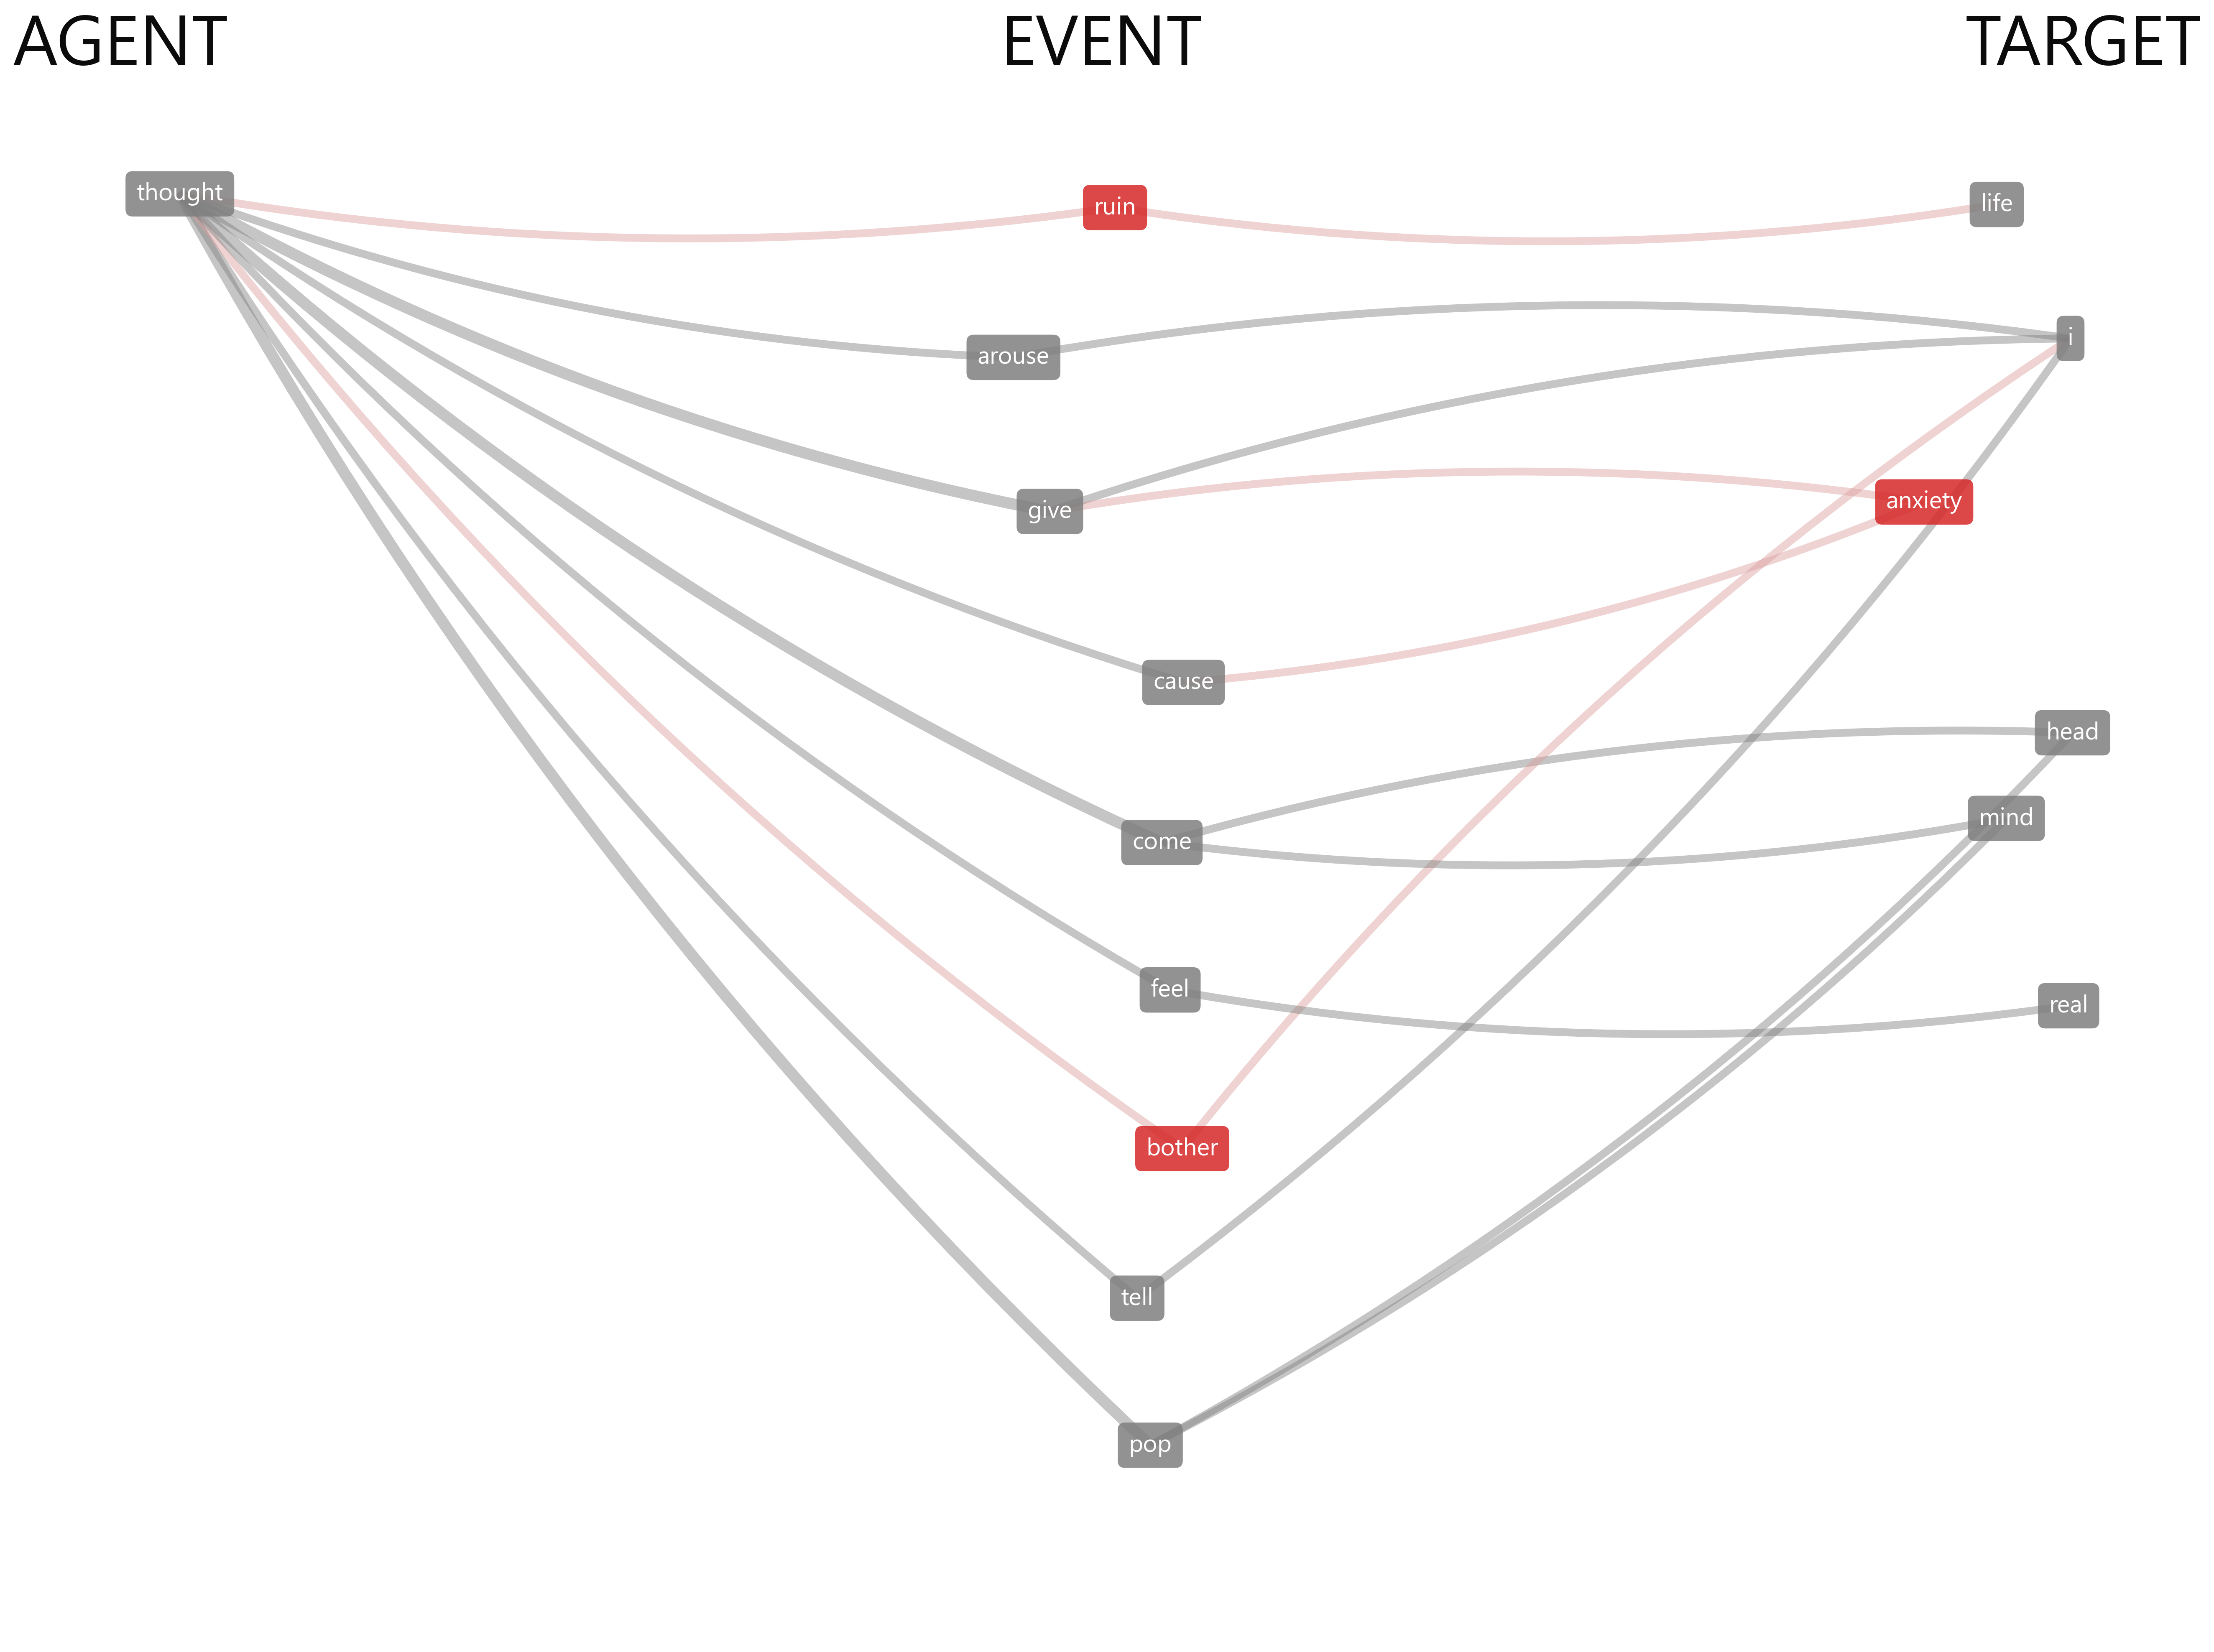
\includegraphics[width=\textwidth]{figures/fig2_tea_OCD_thought.png}
\caption{r/OCD, agent \textit{thought}}
\end{subfigure}
\caption{The twelve most frequent event--target pairs for the agent \textit{he} in r/ptsd and \textit{thought} in r/OCD, counted as number of posts over each full community and drawn with \texttt{plot\_svo\_graph}. Pairs with no target, with the light verbs \textit{be, do, have, get}, with generic targets (\textit{it, what, thing}, etc.) or appearing in fewer than five posts were excluded, as were agentless passives. Events are lemmatised verb heads; ``i'' is the lemmatised narrator (\textit{me}). Node colour shows sentiment valence.}
\label{fig:networks}
\end{figure}

\subsection{Robustness}

None of the checks changed the picture. The agency profiles were essentially the same when passive sentences were reclassified, when each author contributed only one post, and when the sample was split in two at random.

\paragraph{Passive voice.} Agentless passives were rare: they made up 3.3\% (r/OCD) to 4.3\% (r/ptsd) of the self's subject slots, and the differences between communities were small ($|g| \leq 0.21$). Among agentless passives with the narrator as subject and a lexical verb, the most frequent was the same in every community: ``I was diagnosed'', which appeared in 19.5\% of r/ADHD posts and in 5.6--11.9\% of the others. Passives of abuse, rape and triggering were characteristic of r/ptsd but each occurred in only 2--3\% of its posts. The correction therefore changed little. The odds ratio for the self in r/ptsd went from 0.59 to 0.62, the one for person nouns stayed at 1.44, and the one for the self in r/ADHD, where ``I was diagnosed'' is most common, went from 1.43 to 1.32. The reduced agency of the narrator in r/ptsd is not a by-product of passive constructions. It comes from active clauses in which other people are the subject and the narrator is the object.

\paragraph{Authors.} Clustering by post instead of by author gave the same odds ratios and almost identical $p$-values. Keeping one post per author (9,353 posts) changed the odds ratios by at most 0.05. Every effect that was significant in the main analysis remained significant, and none of the others became significant.

\paragraph{Split halves.} Fitted separately on two random halves of the posts, the log odds ratios correlated at $r = .88$ across all category--community cells. For the self, person nouns and \textit{they}, the two halves gave odds ratios of 0.63 and 0.60 (self, r/ptsd), 1.43 and 1.44 (persons, r/ptsd), 1.32 and 1.28 (self, r/OCD) and 0.68 and 0.65 (persons, r/OCD).

% =====================================================================
\section{Discussion}

We start from the agency profiles, because they are where TEA networks added something that word counts could not, and compare each one with what cognitive models of the condition would lead one to expect.

\subsection{Agency profiles and clinical models}

The r/ptsd profile fits the cognitive model of PTSD closely. Ehlers and Clark describe mental defeat as the perceived loss of all autonomy during the trauma, a state in which the person stops experiencing themselves as someone with a will of their own \citep{ehlers2000}. Posts in r/ptsd mention the self as often as posts in r/OCD and r/ADHD, but give it the agent role substantially less often, and they give that role to other people, usually named by their relationship to the narrator (father, boyfriend) or by a pronoun. The effect does not come from passive sentences such as ``I was assaulted'', which are rare. It comes from active sentences in which someone else is the subject. Grammatically, these narratives are told from the position of the person affected. This complements the analysis of r/sexualassault by \citet{abramski2024}, who linked passive-voice narratives to concepts of psychological distress. In our data the passive voice was rare, and the loss of agency showed up mainly in who was made the subject of active clauses. Their observation that family members were more central in active-voice narratives fits the same picture, although the two studies used different units of analysis and cannot be compared directly.

The r/OCD profile points in the other direction and fits cognitive accounts of the disorder in two ways. The self is an agent more often than elsewhere, which matches the inflated sense of responsibility that \citet{salkovskis1985} placed at the centre of obsessional problems: the narrator checks, washes, avoids and neutralises. Other people, by contrast, rarely act. The second feature is that thoughts, the mind and memories are cast as agents more often than in the other communities. This is the grammatical counterpart of the way intrusive thoughts are experienced as alien and consequential \citep{rachman1997}, and of thought-action fusion, the belief that a thought can by itself make harm more likely \citep{shafran1996}.

There is a second reading of the agentive mind that we cannot rule out. A widely used self-help programme for OCD teaches people to relabel intrusive urges as symptoms and then to reattribute them to the brain rather than to themselves \citep{schwartz1996}. Posters who have taken up this framing, from that book or from therapy, would write sentences in which the brain, the thought or the OCD is the subject, and \textit{brain} is indeed the fourth most distinctive agent in r/OCD (Figure~\ref{fig:content}). If part of the effect is learned from treatment, it tells us how recovery language circulates in an online community as much as how obsessions are experienced. These data cannot separate the two.

The r/depression profile is less about persons and more about scope. Absolutist pronouns were more agentive than elsewhere, in line with the finding that absolutist language is elevated in depression \citep{almosaiwi2018}; here the extra information is that ``nothing'', ``everyone'' and ``nobody'' are used as the ones who act (nothing helps, nobody cares). Time is the other distinctive agent: days, years and the future do things to the narrator. The self is mentioned more often in r/depression than anywhere else, consistent with the self-focus literature \citep{rude2004,tackman2019}, but it is not more agentive. Its slightly lower agentivity (OR = 0.94) points in the same direction as the higher rate of passive voice in r/depression reported by \citet{simchon2023} and the lower agency scores of depression-related posts in \citet{witkowska2026}, although the effect here is small.

The r/ADHD profile reflects how the condition is discussed online as much as the condition itself. Medication and the body act on the narrator more often than in the other communities, and ``I was diagnosed'' is by far the most common agentless passive. The self is nonetheless as agentive as in r/OCD. One reading, consistent with accounts of ADHD as a problem of self-regulation \citep{barkley1997}, is that posters describe their own efforts (to focus, start, finish, study) alongside an external regulator, the medication, that helps or fails to help them do so.

\subsection{Thematic concentration}

The recurrence analysis gives a second, independent description of two of the communities. Posts in r/OCD were the most concentrated: their sentences stayed close to one another in meaning, as one would expect when an obsession takes over most of what a person writes about. Posts in r/depression were the least concentrated and moved between many subjects; in the content and agency analyses the same community favoured broad entities such as \textit{life}, \textit{world}, \textit{everything} and \textit{the future}, so the two results describe the same diffuseness from different angles. Rumination is often described as repetitive \citep{nolenhoeksema2000}, and one might have expected r/depression to be the most recurrent community. In these posts the repetition, if present, did not take the form of sentences with similar content. Once each post's recurrence rate was fixed, the sequential measures did not differ, so the effect lies in how homogeneous a post is.

\subsection{What roles add}

It would be easy to present TEA networks as a better feature set for detecting conditions from text; on these data they are not. Roles were informative for a different purpose. The agentivity models condition on mention, so they ask how a community talks about an entity, whatever the frequency of mention. The clearest case is the self: three of the four communities mention it at the same rate, yet they distribute its agency differently, and the differences line up with what clinical theory predicts. A frequency-based measure cannot see this difference, because the frequency is the same, and neither can a measure that treats agency as a property of the whole text, such as a passive-voice rate \citep{simchon2023} or a model-based agency score \citep{witkowska2026}. TEA networks are therefore better suited to describing narratives than to classifying them, and the agency profiles they yield are directly interpretable in the vocabulary of narrative psychology \citep{mcadams1996,adler2012}.

\subsection{Limitations}

The data are posts to online communities, not clinical samples. Membership in a subreddit does not establish a diagnosis, people with comorbid conditions may post in several communities, and posting is shaped by the norms of each community: a community organised around trauma will produce stories about other people's actions partly because that is what members come to share. The profiles therefore describe how these communities write, not how individuals with each diagnosis think.

Most posts date from 2021, during the COVID-19 pandemic, when activity and content in mental health communities shifted \citep{low2020}. Whether the profiles hold in other periods and on other platforms needs to be tested.

Agency is approximated by grammar. The subject of an active verb is usually, but not always, the one who acts: ``I received a diagnosis'' and ``my thoughts tell me'' both have grammatical agents that are not prototypical ones \citep{dowty1991}. We addressed the most obvious mismatch, the agentless passive, and found it made little difference, but other constructions (experiencer subjects, light verbs) remain. Parsing informal text introduces further errors, and coreference was not resolved, so a pronoun is counted under its pronoun class rather than under the entity it refers to.

The category system has its own noise. WordNet supersenses were assigned from the most frequent sense, which misfiles some words (``med'' as communication, ``thing'' as state). The taxonomy was chosen in advance and applied identically to all communities, so this noise should weaken differences rather than create them, but finer categories would sharpen the picture.

The recurrence results depend on how sentences are represented. Two sentence-transformer models and three thresholds gave the same pattern, but both models were trained on general-purpose text, and the 373 posts with fewer than ten sentences after segmentation could not be analysed.

Finally, effects are moderate. The odds ratios range from about 0.6 to 1.5, and the structural differences are small. With ten thousand posts even small differences are estimated precisely; we have therefore emphasised effects that are both large enough to matter and stable across halves of the data, rather than statistical significance alone.

\subsection{Future directions}

Three extensions follow directly. The first is to replicate the profiles in data with clinical information, such as therapy transcripts or narratives from diagnosed patients, and to test whether a person's agency profile changes over treatment, as narrated agency does in coded therapy narratives \citep{adler2012}. The second is to resolve coreference, so that the agentivity of specific people (a parent, a partner, a therapist) can be followed through a story. The third is to look at what agents do as well as who they are: the events attached to an agentive ``thought'' in r/OCD, or to an agentive ``he'' in r/ptsd, carry the content of the appraisal itself.

% =====================================================================
\section{Conclusion}

We asked who acts in the stories people tell in four online mental health communities, using a method that records, for every sentence, who does what to whom. Grammatical roles did not help to tell the communities apart, which plain word counts already do well. They did show something word counts cannot: how each community distributes the role of the one who acts.

In r/ptsd, writers mention themselves as often as anywhere else but are more often the ones acted upon, and other people, often named by their relationship to the writer, are more often the ones acting. In r/OCD the writer is the one acting even more often than elsewhere, other people act less often, and thoughts act more often than in any other community; these posts also stay closest to a single theme. In r/depression, time and sweeping words such as ``nothing'' and ``nobody'' take the active role, and the posts range over more subjects than in any other community. In r/ADHD, the writer acts often alongside medication and the body. The PTSD and OCD patterns resemble what cognitive models of these conditions would predict: the loss of autonomy described in PTSD, and the inflated responsibility and powerful thoughts described in OCD.

For psychologists, the method offers a way to measure narrated agency, a construct usually coded by hand, across thousands of texts and separately for the self, other people and abstract forces. The effects are moderate and the data come from online communities without clinical assessment. Whether the profiles belong to the conditions or to the ways each community has learned to tell its stories is a question the present data leave open.

% =====================================================================
\section*{Data and code availability}

The posts are available from the Hugging Face dataset \texttt{solomonk/reddit\_mental\_health\_posts}. Analysis scripts, derived tables and figure code are available at \url{https://github.com/Jacoposchenetti/Psychiatric_text}. TEA networks were extracted with the TEA\_Networks library (\url{https://github.com/MassimoStel/TEA_Networks}).

\bibliography{references}

\end{document}
